% Created by tikzDevice version 0.10.1 on 2016-07-18 15:18:42
% !TEX encoding = UTF-8 Unicode
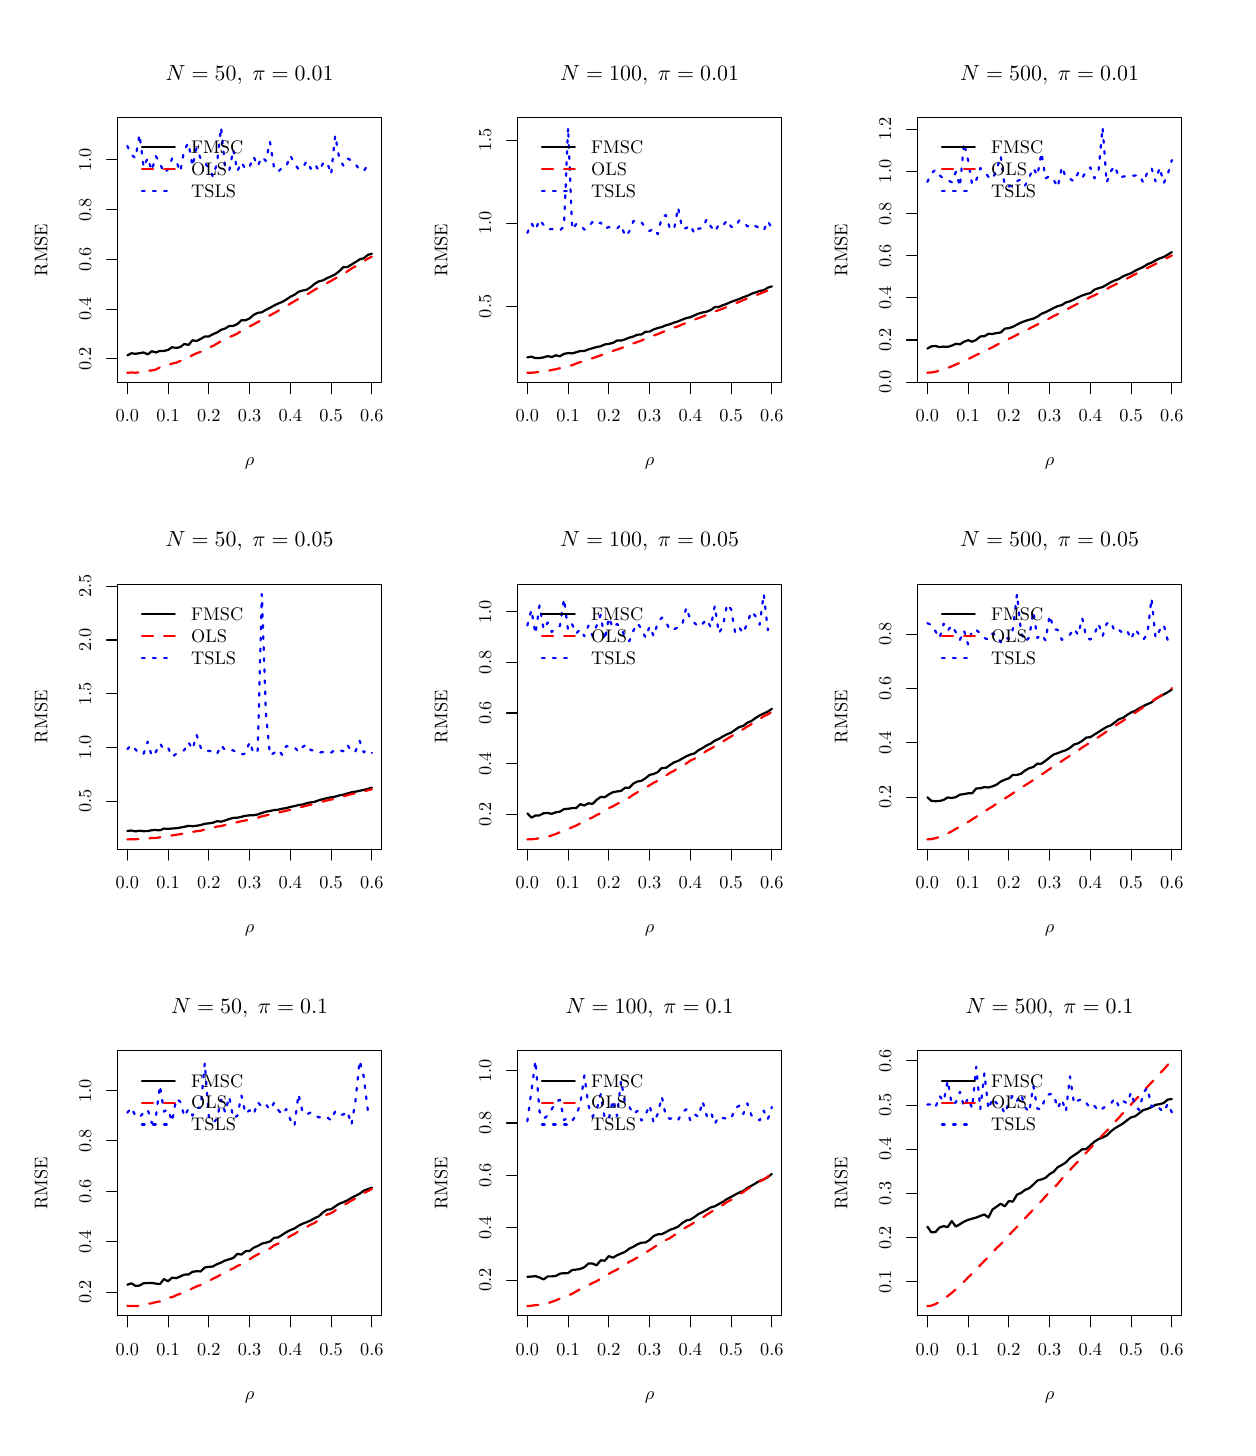
\begin{tikzpicture}[x=1pt,y=1pt]
\definecolor{fillColor}{RGB}{255,255,255}
\path[use as bounding box,fill=fillColor,fill opacity=0.00] (0,0) rectangle (433.62,505.89);
\begin{scope}
\path[clip] ( 32.47,377.65) rectangle (127.91,473.42);
\definecolor{drawColor}{RGB}{0,0,0}

\path[draw=drawColor,line width= 0.8pt,line join=round,line cap=round] ( 36.01,387.44) --
	( 37.48,388.24) --
	( 38.95,388.03) --
	( 40.42,388.27) --
	( 41.90,388.52) --
	( 43.37,387.83) --
	( 44.84,388.97) --
	( 46.32,388.51) --
	( 47.79,389.10) --
	( 49.26,389.06) --
	( 50.73,389.45) --
	( 52.21,390.43) --
	( 53.68,390.14) --
	( 55.15,390.49) --
	( 56.63,391.61) --
	( 58.10,391.24) --
	( 59.57,392.92) --
	( 61.04,392.65) --
	( 62.52,393.43) --
	( 63.99,394.26) --
	( 65.46,394.31) --
	( 66.93,395.12) --
	( 68.41,395.73) --
	( 69.88,396.69) --
	( 71.35,397.18) --
	( 72.83,398.07) --
	( 74.30,398.13) --
	( 75.77,398.78) --
	( 77.24,400.16) --
	( 78.72,400.14) --
	( 80.19,400.84) --
	( 81.66,402.11) --
	( 83.14,402.83) --
	( 84.61,403.04) --
	( 86.08,403.92) --
	( 87.55,404.64) --
	( 89.03,405.47) --
	( 90.50,406.19) --
	( 91.97,406.78) --
	( 93.44,407.64) --
	( 94.92,408.65) --
	( 96.39,409.36) --
	( 97.86,410.45) --
	( 99.34,410.90) --
	(100.81,411.18) --
	(102.28,412.12) --
	(103.75,413.39) --
	(105.23,414.22) --
	(106.70,414.58) --
	(108.17,415.37) --
	(109.65,416.03) --
	(111.12,416.74) --
	(112.59,417.90) --
	(114.06,419.32) --
	(115.54,419.40) --
	(117.01,420.28) --
	(118.48,421.19) --
	(119.95,422.16) --
	(121.43,422.55) --
	(122.90,423.77) --
	(124.37,424.21);
\end{scope}
\begin{scope}
\path[clip] (  0.00,  0.00) rectangle (433.62,505.89);
\definecolor{drawColor}{RGB}{0,0,0}

\path[draw=drawColor,line width= 0.4pt,line join=round,line cap=round] ( 36.01,377.65) -- (124.37,377.65);

\path[draw=drawColor,line width= 0.4pt,line join=round,line cap=round] ( 36.01,377.65) -- ( 36.01,373.69);

\path[draw=drawColor,line width= 0.4pt,line join=round,line cap=round] ( 50.73,377.65) -- ( 50.73,373.69);

\path[draw=drawColor,line width= 0.4pt,line join=round,line cap=round] ( 65.46,377.65) -- ( 65.46,373.69);

\path[draw=drawColor,line width= 0.4pt,line join=round,line cap=round] ( 80.19,377.65) -- ( 80.19,373.69);

\path[draw=drawColor,line width= 0.4pt,line join=round,line cap=round] ( 94.92,377.65) -- ( 94.92,373.69);

\path[draw=drawColor,line width= 0.4pt,line join=round,line cap=round] (109.65,377.65) -- (109.65,373.69);

\path[draw=drawColor,line width= 0.4pt,line join=round,line cap=round] (124.37,377.65) -- (124.37,373.69);

\node[text=drawColor,anchor=base,inner sep=0pt, outer sep=0pt, scale=  0.66] at ( 36.01,363.40) {0.0};

\node[text=drawColor,anchor=base,inner sep=0pt, outer sep=0pt, scale=  0.66] at ( 50.73,363.40) {0.1};

\node[text=drawColor,anchor=base,inner sep=0pt, outer sep=0pt, scale=  0.66] at ( 65.46,363.40) {0.2};

\node[text=drawColor,anchor=base,inner sep=0pt, outer sep=0pt, scale=  0.66] at ( 80.19,363.40) {0.3};

\node[text=drawColor,anchor=base,inner sep=0pt, outer sep=0pt, scale=  0.66] at ( 94.92,363.40) {0.4};

\node[text=drawColor,anchor=base,inner sep=0pt, outer sep=0pt, scale=  0.66] at (109.65,363.40) {0.5};

\node[text=drawColor,anchor=base,inner sep=0pt, outer sep=0pt, scale=  0.66] at (124.37,363.40) {0.6};

\path[draw=drawColor,line width= 0.4pt,line join=round,line cap=round] ( 32.47,386.18) -- ( 32.47,458.10);

\path[draw=drawColor,line width= 0.4pt,line join=round,line cap=round] ( 32.47,386.18) -- ( 28.51,386.18);

\path[draw=drawColor,line width= 0.4pt,line join=round,line cap=round] ( 32.47,404.16) -- ( 28.51,404.16);

\path[draw=drawColor,line width= 0.4pt,line join=round,line cap=round] ( 32.47,422.14) -- ( 28.51,422.14);

\path[draw=drawColor,line width= 0.4pt,line join=round,line cap=round] ( 32.47,440.12) -- ( 28.51,440.12);

\path[draw=drawColor,line width= 0.4pt,line join=round,line cap=round] ( 32.47,458.10) -- ( 28.51,458.10);

\node[text=drawColor,rotate= 90.00,anchor=base,inner sep=0pt, outer sep=0pt, scale=  0.66] at ( 22.97,386.18) {0.2};

\node[text=drawColor,rotate= 90.00,anchor=base,inner sep=0pt, outer sep=0pt, scale=  0.66] at ( 22.97,404.16) {0.4};

\node[text=drawColor,rotate= 90.00,anchor=base,inner sep=0pt, outer sep=0pt, scale=  0.66] at ( 22.97,422.14) {0.6};

\node[text=drawColor,rotate= 90.00,anchor=base,inner sep=0pt, outer sep=0pt, scale=  0.66] at ( 22.97,440.12) {0.8};

\node[text=drawColor,rotate= 90.00,anchor=base,inner sep=0pt, outer sep=0pt, scale=  0.66] at ( 22.97,458.10) {1.0};

\path[draw=drawColor,line width= 0.4pt,line join=round,line cap=round] ( 32.47,377.65) --
	(127.91,377.65) --
	(127.91,473.42) --
	( 32.47,473.42) --
	( 32.47,377.65);
\end{scope}
\begin{scope}
\path[clip] (  0.00,337.26) rectangle (144.54,505.89);
\definecolor{drawColor}{RGB}{0,0,0}

\node[text=drawColor,anchor=base,inner sep=0pt, outer sep=0pt, scale=  0.79] at ( 80.19,486.92) {\bfseries $N=50, \;\pi=0.01$};

\node[text=drawColor,anchor=base,inner sep=0pt, outer sep=0pt, scale=  0.66] at ( 80.19,347.56) {$\rho$};

\node[text=drawColor,rotate= 90.00,anchor=base,inner sep=0pt, outer sep=0pt, scale=  0.66] at (  7.13,425.53) {RMSE};
\end{scope}
\begin{scope}
\path[clip] ( 32.47,377.65) rectangle (127.91,473.42);
\definecolor{drawColor}{RGB}{255,0,0}

\path[draw=drawColor,line width= 0.8pt,dash pattern=on 4pt off 4pt ,line join=round,line cap=round] ( 36.01,381.20) --
	( 37.48,381.26) --
	( 38.95,381.21) --
	( 40.42,381.32) --
	( 41.90,381.63) --
	( 43.37,381.87) --
	( 44.84,382.04) --
	( 46.32,382.34) --
	( 47.79,383.16) --
	( 49.26,383.31) --
	( 50.73,384.03) --
	( 52.21,384.52) --
	( 53.68,384.82) --
	( 55.15,385.45) --
	( 56.63,386.11) --
	( 58.10,386.69) --
	( 59.57,387.56) --
	( 61.04,388.22) --
	( 62.52,388.76) --
	( 63.99,389.47) --
	( 65.46,390.31) --
	( 66.93,390.84) --
	( 68.41,391.73) --
	( 69.88,392.61) --
	( 71.35,393.24) --
	( 72.83,394.06) --
	( 74.30,394.64) --
	( 75.77,395.34) --
	( 77.24,396.39) --
	( 78.72,397.12) --
	( 80.19,397.96) --
	( 81.66,398.69) --
	( 83.14,399.51) --
	( 84.61,400.24) --
	( 86.08,401.22) --
	( 87.55,401.94) --
	( 89.03,402.72) --
	( 90.50,403.56) --
	( 91.97,404.43) --
	( 93.44,405.25) --
	( 94.92,406.17) --
	( 96.39,407.05) --
	( 97.86,407.89) --
	( 99.34,408.68) --
	(100.81,409.29) --
	(102.28,410.31) --
	(103.75,411.20) --
	(105.23,412.03) --
	(106.70,412.76) --
	(108.17,413.61) --
	(109.65,414.41) --
	(111.12,415.27) --
	(112.59,416.19) --
	(114.06,417.14) --
	(115.54,417.81) --
	(117.01,418.84) --
	(118.48,419.67) --
	(119.95,420.64) --
	(121.43,421.46) --
	(122.90,422.42) --
	(124.37,423.17);
\definecolor{drawColor}{RGB}{0,0,255}

\path[draw=drawColor,line width= 0.8pt,dash pattern=on 1pt off 3pt ,line join=round,line cap=round] ( 36.01,463.18) --
	( 37.48,459.93) --
	( 38.95,458.78) --
	( 40.42,467.28) --
	( 41.90,455.45) --
	( 43.37,458.84) --
	( 44.84,454.20) --
	( 46.32,459.47) --
	( 47.79,456.96) --
	( 49.26,453.36) --
	( 50.73,454.72) --
	( 52.21,458.67) --
	( 53.68,457.68) --
	( 55.15,453.88) --
	( 56.63,461.89) --
	( 58.10,464.21) --
	( 59.57,455.80) --
	( 61.04,462.43) --
	( 62.52,458.46) --
	( 63.99,457.11) --
	( 65.46,455.09) --
	( 66.93,452.12) --
	( 68.41,456.85) --
	( 69.88,469.87) --
	( 71.35,455.18) --
	( 72.83,454.19) --
	( 74.30,461.84) --
	( 75.77,454.03) --
	( 77.24,457.24) --
	( 78.72,454.73) --
	( 80.19,455.67) --
	( 81.66,459.26) --
	( 83.14,455.89) --
	( 84.61,459.17) --
	( 86.08,457.75) --
	( 87.55,464.66) --
	( 89.03,455.29) --
	( 90.50,453.79) --
	( 91.97,455.34) --
	( 93.44,455.71) --
	( 94.92,459.70) --
	( 96.39,456.77) --
	( 97.86,454.78) --
	( 99.34,455.15) --
	(100.81,457.66) --
	(102.28,454.92) --
	(103.75,456.66) --
	(105.23,454.13) --
	(106.70,456.80) --
	(108.17,457.38) --
	(109.65,452.89) --
	(111.12,466.97) --
	(112.59,458.64) --
	(114.06,456.06) --
	(115.54,458.66) --
	(117.01,457.85) --
	(118.48,456.54) --
	(119.95,454.48) --
	(121.43,454.06) --
	(122.90,456.26) --
	(124.37,456.56);
\definecolor{drawColor}{RGB}{0,0,0}

\path[draw=drawColor,line width= 0.8pt,line join=round,line cap=round] ( 41.28,462.63) -- ( 53.16,462.63);
\definecolor{drawColor}{RGB}{255,0,0}

\path[draw=drawColor,line width= 0.8pt,dash pattern=on 4pt off 4pt ,line join=round,line cap=round] ( 41.28,454.71) -- ( 53.16,454.71);
\definecolor{drawColor}{RGB}{0,0,255}

\path[draw=drawColor,line width= 0.8pt,dash pattern=on 1pt off 3pt ,line join=round,line cap=round] ( 41.28,446.79) -- ( 53.16,446.79);
\definecolor{drawColor}{RGB}{0,0,0}

\node[text=drawColor,anchor=base west,inner sep=0pt, outer sep=0pt, scale=  0.66] at ( 59.10,460.35) {FMSC};

\node[text=drawColor,anchor=base west,inner sep=0pt, outer sep=0pt, scale=  0.66] at ( 59.10,452.43) {OLS};

\node[text=drawColor,anchor=base west,inner sep=0pt, outer sep=0pt, scale=  0.66] at ( 59.10,444.51) {TSLS};
\end{scope}
\begin{scope}
\path[clip] (177.01,377.65) rectangle (272.45,473.42);
\definecolor{drawColor}{RGB}{0,0,0}

\path[draw=drawColor,line width= 0.8pt,line join=round,line cap=round] (180.55,386.74) --
	(182.02,386.99) --
	(183.49,386.49) --
	(184.96,386.50) --
	(186.44,386.74) --
	(187.91,387.21) --
	(189.38,386.87) --
	(190.86,387.50) --
	(192.33,387.15) --
	(193.80,388.03) --
	(195.27,388.31) --
	(196.75,388.18) --
	(198.22,388.60) --
	(199.69,389.07) --
	(201.17,389.08) --
	(202.64,389.63) --
	(204.11,390.06) --
	(205.58,390.48) --
	(207.06,390.76) --
	(208.53,391.42) --
	(210.00,391.63) --
	(211.47,391.96) --
	(212.95,392.83) --
	(214.42,392.82) --
	(215.89,393.26) --
	(217.37,393.88) --
	(218.84,394.29) --
	(220.31,394.94) --
	(221.78,395.02) --
	(223.26,396.03) --
	(224.73,396.06) --
	(226.20,396.85) --
	(227.68,397.36) --
	(229.15,397.71) --
	(230.62,398.34) --
	(232.09,398.74) --
	(233.57,399.31) --
	(235.04,399.76) --
	(236.51,400.38) --
	(237.98,400.93) --
	(239.46,401.27) --
	(240.93,401.92) --
	(242.40,402.56) --
	(243.88,402.97) --
	(245.35,403.26) --
	(246.82,403.87) --
	(248.29,404.92) --
	(249.77,404.99) --
	(251.24,405.62) --
	(252.71,406.13) --
	(254.19,406.81) --
	(255.66,407.33) --
	(257.13,407.84) --
	(258.60,408.50) --
	(260.08,409.01) --
	(261.55,409.72) --
	(263.02,410.21) --
	(264.50,410.77) --
	(265.97,411.01) --
	(267.44,411.93) --
	(268.91,412.41);
\end{scope}
\begin{scope}
\path[clip] (  0.00,  0.00) rectangle (433.62,505.89);
\definecolor{drawColor}{RGB}{0,0,0}

\path[draw=drawColor,line width= 0.4pt,line join=round,line cap=round] (180.55,377.65) -- (268.91,377.65);

\path[draw=drawColor,line width= 0.4pt,line join=round,line cap=round] (180.55,377.65) -- (180.55,373.69);

\path[draw=drawColor,line width= 0.4pt,line join=round,line cap=round] (195.27,377.65) -- (195.27,373.69);

\path[draw=drawColor,line width= 0.4pt,line join=round,line cap=round] (210.00,377.65) -- (210.00,373.69);

\path[draw=drawColor,line width= 0.4pt,line join=round,line cap=round] (224.73,377.65) -- (224.73,373.69);

\path[draw=drawColor,line width= 0.4pt,line join=round,line cap=round] (239.46,377.65) -- (239.46,373.69);

\path[draw=drawColor,line width= 0.4pt,line join=round,line cap=round] (254.19,377.65) -- (254.19,373.69);

\path[draw=drawColor,line width= 0.4pt,line join=round,line cap=round] (268.91,377.65) -- (268.91,373.69);

\node[text=drawColor,anchor=base,inner sep=0pt, outer sep=0pt, scale=  0.66] at (180.55,363.40) {0.0};

\node[text=drawColor,anchor=base,inner sep=0pt, outer sep=0pt, scale=  0.66] at (195.27,363.40) {0.1};

\node[text=drawColor,anchor=base,inner sep=0pt, outer sep=0pt, scale=  0.66] at (210.00,363.40) {0.2};

\node[text=drawColor,anchor=base,inner sep=0pt, outer sep=0pt, scale=  0.66] at (224.73,363.40) {0.3};

\node[text=drawColor,anchor=base,inner sep=0pt, outer sep=0pt, scale=  0.66] at (239.46,363.40) {0.4};

\node[text=drawColor,anchor=base,inner sep=0pt, outer sep=0pt, scale=  0.66] at (254.19,363.40) {0.5};

\node[text=drawColor,anchor=base,inner sep=0pt, outer sep=0pt, scale=  0.66] at (268.91,363.40) {0.6};

\path[draw=drawColor,line width= 0.4pt,line join=round,line cap=round] (177.01,405.16) -- (177.01,465.26);

\path[draw=drawColor,line width= 0.4pt,line join=round,line cap=round] (177.01,405.16) -- (173.05,405.16);

\path[draw=drawColor,line width= 0.4pt,line join=round,line cap=round] (177.01,435.21) -- (173.05,435.21);

\path[draw=drawColor,line width= 0.4pt,line join=round,line cap=round] (177.01,465.26) -- (173.05,465.26);

\node[text=drawColor,rotate= 90.00,anchor=base,inner sep=0pt, outer sep=0pt, scale=  0.66] at (167.51,405.16) {0.5};

\node[text=drawColor,rotate= 90.00,anchor=base,inner sep=0pt, outer sep=0pt, scale=  0.66] at (167.51,435.21) {1.0};

\node[text=drawColor,rotate= 90.00,anchor=base,inner sep=0pt, outer sep=0pt, scale=  0.66] at (167.51,465.26) {1.5};

\path[draw=drawColor,line width= 0.4pt,line join=round,line cap=round] (177.01,377.65) --
	(272.45,377.65) --
	(272.45,473.42) --
	(177.01,473.42) --
	(177.01,377.65);
\end{scope}
\begin{scope}
\path[clip] (144.54,337.26) rectangle (289.08,505.89);
\definecolor{drawColor}{RGB}{0,0,0}

\node[text=drawColor,anchor=base,inner sep=0pt, outer sep=0pt, scale=  0.79] at (224.73,486.92) {\bfseries $N=100, \;\pi=0.01$};

\node[text=drawColor,anchor=base,inner sep=0pt, outer sep=0pt, scale=  0.66] at (224.73,347.56) {$\rho$};

\node[text=drawColor,rotate= 90.00,anchor=base,inner sep=0pt, outer sep=0pt, scale=  0.66] at (151.67,425.53) {RMSE};
\end{scope}
\begin{scope}
\path[clip] (177.01,377.65) rectangle (272.45,473.42);
\definecolor{drawColor}{RGB}{255,0,0}

\path[draw=drawColor,line width= 0.8pt,dash pattern=on 4pt off 4pt ,line join=round,line cap=round] (180.55,381.20) --
	(182.02,381.20) --
	(183.49,381.31) --
	(184.96,381.48) --
	(186.44,381.60) --
	(187.91,381.79) --
	(189.38,382.21) --
	(190.86,382.47) --
	(192.33,382.82) --
	(193.80,383.19) --
	(195.27,383.57) --
	(196.75,383.94) --
	(198.22,384.53) --
	(199.69,385.04) --
	(201.17,385.51) --
	(202.64,385.92) --
	(204.11,386.44) --
	(205.58,386.96) --
	(207.06,387.45) --
	(208.53,388.03) --
	(210.00,388.58) --
	(211.47,389.07) --
	(212.95,389.58) --
	(214.42,390.07) --
	(215.89,390.60) --
	(217.37,391.28) --
	(218.84,391.79) --
	(220.31,392.32) --
	(221.78,392.83) --
	(223.26,393.52) --
	(224.73,394.13) --
	(226.20,394.62) --
	(227.68,395.16) --
	(229.15,395.78) --
	(230.62,396.38) --
	(232.09,396.85) --
	(233.57,397.51) --
	(235.04,398.00) --
	(236.51,398.65) --
	(237.98,399.19) --
	(239.46,399.84) --
	(240.93,400.38) --
	(242.40,400.93) --
	(243.88,401.50) --
	(245.35,402.05) --
	(246.82,402.61) --
	(248.29,403.30) --
	(249.77,403.84) --
	(251.24,404.39) --
	(252.71,404.97) --
	(254.19,405.65) --
	(255.66,406.27) --
	(257.13,406.77) --
	(258.60,407.45) --
	(260.08,408.00) --
	(261.55,408.64) --
	(263.02,409.12) --
	(264.50,409.74) --
	(265.97,410.32) --
	(267.44,410.92) --
	(268.91,411.54);
\definecolor{drawColor}{RGB}{0,0,255}

\path[draw=drawColor,line width= 0.8pt,dash pattern=on 1pt off 3pt ,line join=round,line cap=round] (180.55,431.72) --
	(182.02,435.22) --
	(183.49,432.80) --
	(184.96,436.51) --
	(186.44,434.56) --
	(187.91,432.99) --
	(189.38,433.12) --
	(190.86,432.97) --
	(192.33,432.64) --
	(193.80,434.03) --
	(195.27,469.87) --
	(196.75,432.97) --
	(198.22,434.90) --
	(199.69,434.76) --
	(201.17,432.87) --
	(202.64,433.82) --
	(204.11,435.70) --
	(205.58,434.63) --
	(207.06,435.47) --
	(208.53,433.22) --
	(210.00,433.83) --
	(211.47,433.47) --
	(212.95,433.27) --
	(214.42,434.75) --
	(215.89,430.47) --
	(217.37,432.18) --
	(218.84,435.90) --
	(220.31,436.38) --
	(221.78,435.56) --
	(223.26,433.69) --
	(224.73,432.38) --
	(226.20,433.36) --
	(227.68,431.26) --
	(229.15,437.49) --
	(230.62,438.14) --
	(232.09,433.21) --
	(233.57,433.05) --
	(235.04,440.93) --
	(236.51,433.27) --
	(237.98,433.44) --
	(239.46,434.60) --
	(240.93,431.44) --
	(242.40,433.30) --
	(243.88,433.42) --
	(245.35,436.70) --
	(246.82,434.10) --
	(248.29,432.15) --
	(249.77,434.75) --
	(251.24,434.24) --
	(252.71,436.32) --
	(254.19,433.95) --
	(255.66,433.76) --
	(257.13,436.25) --
	(258.60,435.55) --
	(260.08,434.07) --
	(261.55,434.99) --
	(263.02,434.15) --
	(264.50,433.59) --
	(265.97,432.58) --
	(267.44,435.97) --
	(268.91,433.42);
\definecolor{drawColor}{RGB}{0,0,0}

\path[draw=drawColor,line width= 0.8pt,line join=round,line cap=round] (185.82,462.63) -- (197.70,462.63);
\definecolor{drawColor}{RGB}{255,0,0}

\path[draw=drawColor,line width= 0.8pt,dash pattern=on 4pt off 4pt ,line join=round,line cap=round] (185.82,454.71) -- (197.70,454.71);
\definecolor{drawColor}{RGB}{0,0,255}

\path[draw=drawColor,line width= 0.8pt,dash pattern=on 1pt off 3pt ,line join=round,line cap=round] (185.82,446.79) -- (197.70,446.79);
\definecolor{drawColor}{RGB}{0,0,0}

\node[text=drawColor,anchor=base west,inner sep=0pt, outer sep=0pt, scale=  0.66] at (203.64,460.35) {FMSC};

\node[text=drawColor,anchor=base west,inner sep=0pt, outer sep=0pt, scale=  0.66] at (203.64,452.43) {OLS};

\node[text=drawColor,anchor=base west,inner sep=0pt, outer sep=0pt, scale=  0.66] at (203.64,444.51) {TSLS};
\end{scope}
\begin{scope}
\path[clip] (321.55,377.65) rectangle (416.99,473.42);
\definecolor{drawColor}{RGB}{0,0,0}

\path[draw=drawColor,line width= 0.8pt,line join=round,line cap=round] (325.09,389.91) --
	(326.56,390.74) --
	(328.03,390.86) --
	(329.50,390.46) --
	(330.98,390.64) --
	(332.45,390.55) --
	(333.92,390.98) --
	(335.40,391.67) --
	(336.87,391.46) --
	(338.34,392.40) --
	(339.81,392.96) --
	(341.29,392.41) --
	(342.76,393.10) --
	(344.23,394.31) --
	(345.71,394.40) --
	(347.18,395.26) --
	(348.65,395.21) --
	(350.12,395.54) --
	(351.60,395.74) --
	(353.07,397.13) --
	(354.54,397.30) --
	(356.01,397.81) --
	(357.49,398.59) --
	(358.96,399.32) --
	(360.43,399.90) --
	(361.91,400.36) --
	(363.38,400.73) --
	(364.85,401.46) --
	(366.32,402.50) --
	(367.80,403.08) --
	(369.27,403.82) --
	(370.74,404.59) --
	(372.22,405.28) --
	(373.69,405.65) --
	(375.16,406.61) --
	(376.63,407.01) --
	(378.11,407.68) --
	(379.58,408.45) --
	(381.05,409.10) --
	(382.52,409.60) --
	(384.00,409.99) --
	(385.47,411.21) --
	(386.94,411.75) --
	(388.42,412.17) --
	(389.89,413.00) --
	(391.36,413.89) --
	(392.83,414.54) --
	(394.31,415.10) --
	(395.78,416.01) --
	(397.25,416.64) --
	(398.73,417.18) --
	(400.20,418.08) --
	(401.67,418.75) --
	(403.14,419.44) --
	(404.62,420.40) --
	(406.09,420.97) --
	(407.56,421.78) --
	(409.04,422.51) --
	(410.51,423.02) --
	(411.98,423.89) --
	(413.45,424.79);
\end{scope}
\begin{scope}
\path[clip] (  0.00,  0.00) rectangle (433.62,505.89);
\definecolor{drawColor}{RGB}{0,0,0}

\path[draw=drawColor,line width= 0.4pt,line join=round,line cap=round] (325.09,377.65) -- (413.45,377.65);

\path[draw=drawColor,line width= 0.4pt,line join=round,line cap=round] (325.09,377.65) -- (325.09,373.69);

\path[draw=drawColor,line width= 0.4pt,line join=round,line cap=round] (339.81,377.65) -- (339.81,373.69);

\path[draw=drawColor,line width= 0.4pt,line join=round,line cap=round] (354.54,377.65) -- (354.54,373.69);

\path[draw=drawColor,line width= 0.4pt,line join=round,line cap=round] (369.27,377.65) -- (369.27,373.69);

\path[draw=drawColor,line width= 0.4pt,line join=round,line cap=round] (384.00,377.65) -- (384.00,373.69);

\path[draw=drawColor,line width= 0.4pt,line join=round,line cap=round] (398.73,377.65) -- (398.73,373.69);

\path[draw=drawColor,line width= 0.4pt,line join=round,line cap=round] (413.45,377.65) -- (413.45,373.69);

\node[text=drawColor,anchor=base,inner sep=0pt, outer sep=0pt, scale=  0.66] at (325.09,363.40) {0.0};

\node[text=drawColor,anchor=base,inner sep=0pt, outer sep=0pt, scale=  0.66] at (339.81,363.40) {0.1};

\node[text=drawColor,anchor=base,inner sep=0pt, outer sep=0pt, scale=  0.66] at (354.54,363.40) {0.2};

\node[text=drawColor,anchor=base,inner sep=0pt, outer sep=0pt, scale=  0.66] at (369.27,363.40) {0.3};

\node[text=drawColor,anchor=base,inner sep=0pt, outer sep=0pt, scale=  0.66] at (384.00,363.40) {0.4};

\node[text=drawColor,anchor=base,inner sep=0pt, outer sep=0pt, scale=  0.66] at (398.73,363.40) {0.5};

\node[text=drawColor,anchor=base,inner sep=0pt, outer sep=0pt, scale=  0.66] at (413.45,363.40) {0.6};

\path[draw=drawColor,line width= 0.4pt,line join=round,line cap=round] (321.55,377.82) -- (321.55,469.18);

\path[draw=drawColor,line width= 0.4pt,line join=round,line cap=round] (321.55,377.82) -- (317.59,377.82);

\path[draw=drawColor,line width= 0.4pt,line join=round,line cap=round] (321.55,393.04) -- (317.59,393.04);

\path[draw=drawColor,line width= 0.4pt,line join=round,line cap=round] (321.55,408.27) -- (317.59,408.27);

\path[draw=drawColor,line width= 0.4pt,line join=round,line cap=round] (321.55,423.50) -- (317.59,423.50);

\path[draw=drawColor,line width= 0.4pt,line join=round,line cap=round] (321.55,438.72) -- (317.59,438.72);

\path[draw=drawColor,line width= 0.4pt,line join=round,line cap=round] (321.55,453.95) -- (317.59,453.95);

\path[draw=drawColor,line width= 0.4pt,line join=round,line cap=round] (321.55,469.18) -- (317.59,469.18);

\node[text=drawColor,rotate= 90.00,anchor=base,inner sep=0pt, outer sep=0pt, scale=  0.66] at (312.05,377.82) {0.0};

\node[text=drawColor,rotate= 90.00,anchor=base,inner sep=0pt, outer sep=0pt, scale=  0.66] at (312.05,393.04) {0.2};

\node[text=drawColor,rotate= 90.00,anchor=base,inner sep=0pt, outer sep=0pt, scale=  0.66] at (312.05,408.27) {0.4};

\node[text=drawColor,rotate= 90.00,anchor=base,inner sep=0pt, outer sep=0pt, scale=  0.66] at (312.05,423.50) {0.6};

\node[text=drawColor,rotate= 90.00,anchor=base,inner sep=0pt, outer sep=0pt, scale=  0.66] at (312.05,438.72) {0.8};

\node[text=drawColor,rotate= 90.00,anchor=base,inner sep=0pt, outer sep=0pt, scale=  0.66] at (312.05,453.95) {1.0};

\node[text=drawColor,rotate= 90.00,anchor=base,inner sep=0pt, outer sep=0pt, scale=  0.66] at (312.05,469.18) {1.2};

\path[draw=drawColor,line width= 0.4pt,line join=round,line cap=round] (321.55,377.65) --
	(416.99,377.65) --
	(416.99,473.42) --
	(321.55,473.42) --
	(321.55,377.65);
\end{scope}
\begin{scope}
\path[clip] (289.08,337.26) rectangle (433.62,505.89);
\definecolor{drawColor}{RGB}{0,0,0}

\node[text=drawColor,anchor=base,inner sep=0pt, outer sep=0pt, scale=  0.79] at (369.27,486.92) {\bfseries $N=500, \;\pi=0.01$};

\node[text=drawColor,anchor=base,inner sep=0pt, outer sep=0pt, scale=  0.66] at (369.27,347.56) {$\rho$};

\node[text=drawColor,rotate= 90.00,anchor=base,inner sep=0pt, outer sep=0pt, scale=  0.66] at (296.21,425.53) {RMSE};
\end{scope}
\begin{scope}
\path[clip] (321.55,377.65) rectangle (416.99,473.42);
\definecolor{drawColor}{RGB}{255,0,0}

\path[draw=drawColor,line width= 0.8pt,dash pattern=on 4pt off 4pt ,line join=round,line cap=round] (325.09,381.20) --
	(326.56,381.31) --
	(328.03,381.55) --
	(329.50,381.96) --
	(330.98,382.39) --
	(332.45,382.91) --
	(333.92,383.52) --
	(335.40,384.16) --
	(336.87,384.81) --
	(338.34,385.44) --
	(339.81,386.09) --
	(341.29,386.86) --
	(342.76,387.61) --
	(344.23,388.28) --
	(345.71,389.01) --
	(347.18,389.72) --
	(348.65,390.45) --
	(350.12,391.21) --
	(351.60,391.92) --
	(353.07,392.65) --
	(354.54,393.42) --
	(356.01,394.12) --
	(357.49,394.90) --
	(358.96,395.64) --
	(360.43,396.45) --
	(361.91,397.12) --
	(363.38,397.89) --
	(364.85,398.62) --
	(366.32,399.43) --
	(367.80,400.15) --
	(369.27,400.86) --
	(370.74,401.68) --
	(372.22,402.40) --
	(373.69,403.16) --
	(375.16,403.90) --
	(376.63,404.70) --
	(378.11,405.47) --
	(379.58,406.20) --
	(381.05,406.91) --
	(382.52,407.71) --
	(384.00,408.53) --
	(385.47,409.17) --
	(386.94,409.93) --
	(388.42,410.69) --
	(389.89,411.46) --
	(391.36,412.28) --
	(392.83,412.97) --
	(394.31,413.70) --
	(395.78,414.47) --
	(397.25,415.25) --
	(398.73,416.04) --
	(400.20,416.81) --
	(401.67,417.54) --
	(403.14,418.29) --
	(404.62,419.03) --
	(406.09,419.81) --
	(407.56,420.51) --
	(409.04,421.30) --
	(410.51,422.08) --
	(411.98,422.83) --
	(413.45,423.54);
\definecolor{drawColor}{RGB}{0,0,255}

\path[draw=drawColor,line width= 0.8pt,dash pattern=on 1pt off 3pt ,line join=round,line cap=round] (325.09,450.14) --
	(326.56,453.21) --
	(328.03,454.54) --
	(329.50,452.50) --
	(330.98,451.40) --
	(332.45,450.66) --
	(333.92,450.08) --
	(335.40,453.79) --
	(336.87,448.50) --
	(338.34,464.24) --
	(339.81,458.00) --
	(341.29,449.08) --
	(342.76,450.76) --
	(344.23,455.14) --
	(345.71,453.99) --
	(347.18,451.99) --
	(348.65,451.11) --
	(350.12,454.52) --
	(351.60,459.51) --
	(353.07,448.48) --
	(354.54,448.55) --
	(356.01,448.74) --
	(357.49,450.42) --
	(358.96,451.07) --
	(360.43,448.86) --
	(361.91,451.86) --
	(363.38,455.18) --
	(364.85,452.46) --
	(366.32,460.68) --
	(367.80,451.45) --
	(369.27,452.24) --
	(370.74,450.88) --
	(372.22,448.23) --
	(373.69,455.60) --
	(375.16,451.73) --
	(376.63,451.29) --
	(378.11,450.31) --
	(379.58,453.40) --
	(381.05,451.51) --
	(382.52,454.08) --
	(384.00,455.38) --
	(385.47,451.44) --
	(386.94,454.11) --
	(388.42,469.87) --
	(389.89,449.84) --
	(391.36,453.97) --
	(392.83,455.93) --
	(394.31,451.70) --
	(395.78,452.07) --
	(397.25,452.27) --
	(398.73,452.31) --
	(400.20,452.47) --
	(401.67,452.67) --
	(403.14,449.85) --
	(404.62,453.74) --
	(406.09,455.24) --
	(407.56,450.36) --
	(409.04,455.33) --
	(410.51,449.68) --
	(411.98,452.96) --
	(413.45,458.07);
\definecolor{drawColor}{RGB}{0,0,0}

\path[draw=drawColor,line width= 0.8pt,line join=round,line cap=round] (330.36,462.63) -- (342.24,462.63);
\definecolor{drawColor}{RGB}{255,0,0}

\path[draw=drawColor,line width= 0.8pt,dash pattern=on 4pt off 4pt ,line join=round,line cap=round] (330.36,454.71) -- (342.24,454.71);
\definecolor{drawColor}{RGB}{0,0,255}

\path[draw=drawColor,line width= 0.8pt,dash pattern=on 1pt off 3pt ,line join=round,line cap=round] (330.36,446.79) -- (342.24,446.79);
\definecolor{drawColor}{RGB}{0,0,0}

\node[text=drawColor,anchor=base west,inner sep=0pt, outer sep=0pt, scale=  0.66] at (348.18,460.35) {FMSC};

\node[text=drawColor,anchor=base west,inner sep=0pt, outer sep=0pt, scale=  0.66] at (348.18,452.43) {OLS};

\node[text=drawColor,anchor=base west,inner sep=0pt, outer sep=0pt, scale=  0.66] at (348.18,444.51) {TSLS};
\end{scope}
\begin{scope}
\path[clip] ( 32.47,209.02) rectangle (127.91,304.79);
\definecolor{drawColor}{RGB}{0,0,0}

\path[draw=drawColor,line width= 0.8pt,line join=round,line cap=round] ( 36.01,215.62) --
	( 37.48,215.77) --
	( 38.95,215.47) --
	( 40.42,215.71) --
	( 41.90,215.55) --
	( 43.37,215.56) --
	( 44.84,215.90) --
	( 46.32,215.96) --
	( 47.79,215.83) --
	( 49.26,216.49) --
	( 50.73,216.36) --
	( 52.21,216.51) --
	( 53.68,216.60) --
	( 55.15,216.85) --
	( 56.63,217.12) --
	( 58.10,217.47) --
	( 59.57,217.33) --
	( 61.04,217.50) --
	( 62.52,217.75) --
	( 63.99,218.22) --
	( 65.46,218.36) --
	( 66.93,218.58) --
	( 68.41,219.16) --
	( 69.88,218.97) --
	( 71.35,219.42) --
	( 72.83,219.94) --
	( 74.30,220.34) --
	( 75.77,220.42) --
	( 77.24,220.72) --
	( 78.72,221.09) --
	( 80.19,221.26) --
	( 81.66,221.31) --
	( 83.14,221.59) --
	( 84.61,222.10) --
	( 86.08,222.58) --
	( 87.55,222.85) --
	( 89.03,223.16) --
	( 90.50,223.28) --
	( 91.97,223.67) --
	( 93.44,223.88) --
	( 94.92,224.29) --
	( 96.39,224.60) --
	( 97.86,224.99) --
	( 99.34,225.17) --
	(100.81,225.67) --
	(102.28,225.94) --
	(103.75,226.17) --
	(105.23,226.71) --
	(106.70,227.12) --
	(108.17,227.49) --
	(109.65,227.79) --
	(111.12,228.02) --
	(112.59,228.46) --
	(114.06,228.72) --
	(115.54,229.16) --
	(117.01,229.59) --
	(118.48,229.83) --
	(119.95,230.13) --
	(121.43,230.46) --
	(122.90,230.79) --
	(124.37,231.28);
\end{scope}
\begin{scope}
\path[clip] (  0.00,  0.00) rectangle (433.62,505.89);
\definecolor{drawColor}{RGB}{0,0,0}

\path[draw=drawColor,line width= 0.4pt,line join=round,line cap=round] ( 36.01,209.02) -- (124.37,209.02);

\path[draw=drawColor,line width= 0.4pt,line join=round,line cap=round] ( 36.01,209.02) -- ( 36.01,205.06);

\path[draw=drawColor,line width= 0.4pt,line join=round,line cap=round] ( 50.73,209.02) -- ( 50.73,205.06);

\path[draw=drawColor,line width= 0.4pt,line join=round,line cap=round] ( 65.46,209.02) -- ( 65.46,205.06);

\path[draw=drawColor,line width= 0.4pt,line join=round,line cap=round] ( 80.19,209.02) -- ( 80.19,205.06);

\path[draw=drawColor,line width= 0.4pt,line join=round,line cap=round] ( 94.92,209.02) -- ( 94.92,205.06);

\path[draw=drawColor,line width= 0.4pt,line join=round,line cap=round] (109.65,209.02) -- (109.65,205.06);

\path[draw=drawColor,line width= 0.4pt,line join=round,line cap=round] (124.37,209.02) -- (124.37,205.06);

\node[text=drawColor,anchor=base,inner sep=0pt, outer sep=0pt, scale=  0.66] at ( 36.01,194.77) {0.0};

\node[text=drawColor,anchor=base,inner sep=0pt, outer sep=0pt, scale=  0.66] at ( 50.73,194.77) {0.1};

\node[text=drawColor,anchor=base,inner sep=0pt, outer sep=0pt, scale=  0.66] at ( 65.46,194.77) {0.2};

\node[text=drawColor,anchor=base,inner sep=0pt, outer sep=0pt, scale=  0.66] at ( 80.19,194.77) {0.3};

\node[text=drawColor,anchor=base,inner sep=0pt, outer sep=0pt, scale=  0.66] at ( 94.92,194.77) {0.4};

\node[text=drawColor,anchor=base,inner sep=0pt, outer sep=0pt, scale=  0.66] at (109.65,194.77) {0.5};

\node[text=drawColor,anchor=base,inner sep=0pt, outer sep=0pt, scale=  0.66] at (124.37,194.77) {0.6};

\path[draw=drawColor,line width= 0.4pt,line join=round,line cap=round] ( 32.47,226.38) -- ( 32.47,304.04);

\path[draw=drawColor,line width= 0.4pt,line join=round,line cap=round] ( 32.47,226.38) -- ( 28.51,226.38);

\path[draw=drawColor,line width= 0.4pt,line join=round,line cap=round] ( 32.47,245.80) -- ( 28.51,245.80);

\path[draw=drawColor,line width= 0.4pt,line join=round,line cap=round] ( 32.47,265.21) -- ( 28.51,265.21);

\path[draw=drawColor,line width= 0.4pt,line join=round,line cap=round] ( 32.47,284.63) -- ( 28.51,284.63);

\path[draw=drawColor,line width= 0.4pt,line join=round,line cap=round] ( 32.47,304.04) -- ( 28.51,304.04);

\node[text=drawColor,rotate= 90.00,anchor=base,inner sep=0pt, outer sep=0pt, scale=  0.66] at ( 22.97,226.38) {0.5};

\node[text=drawColor,rotate= 90.00,anchor=base,inner sep=0pt, outer sep=0pt, scale=  0.66] at ( 22.97,245.80) {1.0};

\node[text=drawColor,rotate= 90.00,anchor=base,inner sep=0pt, outer sep=0pt, scale=  0.66] at ( 22.97,265.21) {1.5};

\node[text=drawColor,rotate= 90.00,anchor=base,inner sep=0pt, outer sep=0pt, scale=  0.66] at ( 22.97,284.63) {2.0};

\node[text=drawColor,rotate= 90.00,anchor=base,inner sep=0pt, outer sep=0pt, scale=  0.66] at ( 22.97,304.04) {2.5};

\path[draw=drawColor,line width= 0.4pt,line join=round,line cap=round] ( 32.47,209.02) --
	(127.91,209.02) --
	(127.91,304.79) --
	( 32.47,304.79) --
	( 32.47,209.02);
\end{scope}
\begin{scope}
\path[clip] (  0.00,168.63) rectangle (144.54,337.26);
\definecolor{drawColor}{RGB}{0,0,0}

\node[text=drawColor,anchor=base,inner sep=0pt, outer sep=0pt, scale=  0.79] at ( 80.19,318.29) {\bfseries $N=50, \;\pi=0.05$};

\node[text=drawColor,anchor=base,inner sep=0pt, outer sep=0pt, scale=  0.66] at ( 80.19,178.93) {$\rho$};

\node[text=drawColor,rotate= 90.00,anchor=base,inner sep=0pt, outer sep=0pt, scale=  0.66] at (  7.13,256.90) {RMSE};
\end{scope}
\begin{scope}
\path[clip] ( 32.47,209.02) rectangle (127.91,304.79);
\definecolor{drawColor}{RGB}{255,0,0}

\path[draw=drawColor,line width= 0.8pt,dash pattern=on 4pt off 4pt ,line join=round,line cap=round] ( 36.01,212.57) --
	( 37.48,212.60) --
	( 38.95,212.65) --
	( 40.42,212.69) --
	( 41.90,212.81) --
	( 43.37,212.93) --
	( 44.84,213.05) --
	( 46.32,213.10) --
	( 47.79,213.33) --
	( 49.26,213.53) --
	( 50.73,213.76) --
	( 52.21,213.99) --
	( 53.68,214.26) --
	( 55.15,214.45) --
	( 56.63,214.73) --
	( 58.10,214.94) --
	( 59.57,215.29) --
	( 61.04,215.53) --
	( 62.52,215.70) --
	( 63.99,216.17) --
	( 65.46,216.39) --
	( 66.93,216.74) --
	( 68.41,217.20) --
	( 69.88,217.37) --
	( 71.35,217.78) --
	( 72.83,218.17) --
	( 74.30,218.46) --
	( 75.77,218.78) --
	( 77.24,219.16) --
	( 78.72,219.41) --
	( 80.19,219.85) --
	( 81.66,220.12) --
	( 83.14,220.41) --
	( 84.61,220.90) --
	( 86.08,221.23) --
	( 87.55,221.57) --
	( 89.03,221.97) --
	( 90.50,222.24) --
	( 91.97,222.59) --
	( 93.44,222.94) --
	( 94.92,223.27) --
	( 96.39,223.72) --
	( 97.86,223.97) --
	( 99.34,224.39) --
	(100.81,224.78) --
	(102.28,225.09) --
	(103.75,225.52) --
	(105.23,225.89) --
	(106.70,226.27) --
	(108.17,226.65) --
	(109.65,226.96) --
	(111.12,227.28) --
	(112.59,227.71) --
	(114.06,228.07) --
	(115.54,228.53) --
	(117.01,228.94) --
	(118.48,229.22) --
	(119.95,229.55) --
	(121.43,229.93) --
	(122.90,230.32) --
	(124.37,230.68);
\definecolor{drawColor}{RGB}{0,0,255}

\path[draw=drawColor,line width= 0.8pt,dash pattern=on 1pt off 3pt ,line join=round,line cap=round] ( 36.01,245.17) --
	( 37.48,246.72) --
	( 38.95,245.11) --
	( 40.42,243.41) --
	( 41.90,243.55) --
	( 43.37,247.88) --
	( 44.84,242.63) --
	( 46.32,244.21) --
	( 47.79,247.19) --
	( 49.26,245.12) --
	( 50.73,245.73) --
	( 52.21,242.43) --
	( 53.68,243.48) --
	( 55.15,243.96) --
	( 56.63,244.87) --
	( 58.10,247.69) --
	( 59.57,245.14) --
	( 61.04,250.35) --
	( 62.52,245.76) --
	( 63.99,244.29) --
	( 65.46,244.57) --
	( 66.93,244.36) --
	( 68.41,243.37) --
	( 69.88,246.62) --
	( 71.35,244.86) --
	( 72.83,244.94) --
	( 74.30,244.74) --
	( 75.77,243.51) --
	( 77.24,243.32) --
	( 78.72,243.58) --
	( 80.19,247.83) --
	( 81.66,243.56) --
	( 83.14,244.71) --
	( 84.61,301.24) --
	( 86.08,258.22) --
	( 87.55,243.04) --
	( 89.03,243.78) --
	( 90.50,244.99) --
	( 91.97,243.14) --
	( 93.44,246.33) --
	( 94.92,245.98) --
	( 96.39,245.95) --
	( 97.86,244.19) --
	( 99.34,245.95) --
	(100.81,246.89) --
	(102.28,244.83) --
	(103.75,244.62) --
	(105.23,243.93) --
	(106.70,244.14) --
	(108.17,244.45) --
	(109.65,243.93) --
	(111.12,244.98) --
	(112.59,244.87) --
	(114.06,244.40) --
	(115.54,246.75) --
	(117.01,244.16) --
	(118.48,244.46) --
	(119.95,248.18) --
	(121.43,244.04) --
	(122.90,244.91) --
	(124.37,243.85);
\definecolor{drawColor}{RGB}{0,0,0}

\path[draw=drawColor,line width= 0.8pt,line join=round,line cap=round] ( 41.28,294.00) -- ( 53.16,294.00);
\definecolor{drawColor}{RGB}{255,0,0}

\path[draw=drawColor,line width= 0.8pt,dash pattern=on 4pt off 4pt ,line join=round,line cap=round] ( 41.28,286.08) -- ( 53.16,286.08);
\definecolor{drawColor}{RGB}{0,0,255}

\path[draw=drawColor,line width= 0.8pt,dash pattern=on 1pt off 3pt ,line join=round,line cap=round] ( 41.28,278.16) -- ( 53.16,278.16);
\definecolor{drawColor}{RGB}{0,0,0}

\node[text=drawColor,anchor=base west,inner sep=0pt, outer sep=0pt, scale=  0.66] at ( 59.10,291.72) {FMSC};

\node[text=drawColor,anchor=base west,inner sep=0pt, outer sep=0pt, scale=  0.66] at ( 59.10,283.80) {OLS};

\node[text=drawColor,anchor=base west,inner sep=0pt, outer sep=0pt, scale=  0.66] at ( 59.10,275.88) {TSLS};
\end{scope}
\begin{scope}
\path[clip] (177.01,209.02) rectangle (272.45,304.79);
\definecolor{drawColor}{RGB}{0,0,0}

\path[draw=drawColor,line width= 0.8pt,line join=round,line cap=round] (180.55,222.00) --
	(182.02,220.45) --
	(183.49,221.19) --
	(184.96,221.25) --
	(186.44,222.02) --
	(187.91,222.12) --
	(189.38,221.82) --
	(190.86,222.37) --
	(192.33,222.59) --
	(193.80,223.51) --
	(195.27,223.63) --
	(196.75,223.86) --
	(198.22,223.92) --
	(199.69,225.29) --
	(201.17,224.83) --
	(202.64,225.62) --
	(204.11,225.40) --
	(205.58,226.85) --
	(207.06,227.92) --
	(208.53,227.82) --
	(210.00,228.84) --
	(211.47,229.62) --
	(212.95,229.89) --
	(214.42,230.10) --
	(215.89,231.26) --
	(217.37,231.19) --
	(218.84,232.73) --
	(220.31,233.48) --
	(221.78,233.73) --
	(223.26,234.66) --
	(224.73,235.87) --
	(226.20,236.21) --
	(227.68,236.90) --
	(229.15,238.39) --
	(230.62,238.42) --
	(232.09,239.45) --
	(233.57,240.40) --
	(235.04,240.93) --
	(236.51,241.75) --
	(237.98,242.59) --
	(239.46,243.23) --
	(240.93,243.63) --
	(242.40,244.80) --
	(243.88,245.60) --
	(245.35,246.53) --
	(246.82,247.20) --
	(248.29,248.26) --
	(249.77,248.88) --
	(251.24,249.80) --
	(252.71,250.57) --
	(254.19,251.15) --
	(255.66,252.18) --
	(257.13,253.16) --
	(258.60,253.58) --
	(260.08,254.76) --
	(261.55,255.34) --
	(263.02,256.45) --
	(264.50,257.36) --
	(265.97,258.07) --
	(267.44,258.75) --
	(268.91,259.75);
\end{scope}
\begin{scope}
\path[clip] (  0.00,  0.00) rectangle (433.62,505.89);
\definecolor{drawColor}{RGB}{0,0,0}

\path[draw=drawColor,line width= 0.4pt,line join=round,line cap=round] (180.55,209.02) -- (268.91,209.02);

\path[draw=drawColor,line width= 0.4pt,line join=round,line cap=round] (180.55,209.02) -- (180.55,205.06);

\path[draw=drawColor,line width= 0.4pt,line join=round,line cap=round] (195.27,209.02) -- (195.27,205.06);

\path[draw=drawColor,line width= 0.4pt,line join=round,line cap=round] (210.00,209.02) -- (210.00,205.06);

\path[draw=drawColor,line width= 0.4pt,line join=round,line cap=round] (224.73,209.02) -- (224.73,205.06);

\path[draw=drawColor,line width= 0.4pt,line join=round,line cap=round] (239.46,209.02) -- (239.46,205.06);

\path[draw=drawColor,line width= 0.4pt,line join=round,line cap=round] (254.19,209.02) -- (254.19,205.06);

\path[draw=drawColor,line width= 0.4pt,line join=round,line cap=round] (268.91,209.02) -- (268.91,205.06);

\node[text=drawColor,anchor=base,inner sep=0pt, outer sep=0pt, scale=  0.66] at (180.55,194.77) {0.0};

\node[text=drawColor,anchor=base,inner sep=0pt, outer sep=0pt, scale=  0.66] at (195.27,194.77) {0.1};

\node[text=drawColor,anchor=base,inner sep=0pt, outer sep=0pt, scale=  0.66] at (210.00,194.77) {0.2};

\node[text=drawColor,anchor=base,inner sep=0pt, outer sep=0pt, scale=  0.66] at (224.73,194.77) {0.3};

\node[text=drawColor,anchor=base,inner sep=0pt, outer sep=0pt, scale=  0.66] at (239.46,194.77) {0.4};

\node[text=drawColor,anchor=base,inner sep=0pt, outer sep=0pt, scale=  0.66] at (254.19,194.77) {0.5};

\node[text=drawColor,anchor=base,inner sep=0pt, outer sep=0pt, scale=  0.66] at (268.91,194.77) {0.6};

\path[draw=drawColor,line width= 0.4pt,line join=round,line cap=round] (177.01,221.63) -- (177.01,294.84);

\path[draw=drawColor,line width= 0.4pt,line join=round,line cap=round] (177.01,221.63) -- (173.05,221.63);

\path[draw=drawColor,line width= 0.4pt,line join=round,line cap=round] (177.01,239.93) -- (173.05,239.93);

\path[draw=drawColor,line width= 0.4pt,line join=round,line cap=round] (177.01,258.24) -- (173.05,258.24);

\path[draw=drawColor,line width= 0.4pt,line join=round,line cap=round] (177.01,276.54) -- (173.05,276.54);

\path[draw=drawColor,line width= 0.4pt,line join=round,line cap=round] (177.01,294.84) -- (173.05,294.84);

\node[text=drawColor,rotate= 90.00,anchor=base,inner sep=0pt, outer sep=0pt, scale=  0.66] at (167.51,221.63) {0.2};

\node[text=drawColor,rotate= 90.00,anchor=base,inner sep=0pt, outer sep=0pt, scale=  0.66] at (167.51,239.93) {0.4};

\node[text=drawColor,rotate= 90.00,anchor=base,inner sep=0pt, outer sep=0pt, scale=  0.66] at (167.51,258.24) {0.6};

\node[text=drawColor,rotate= 90.00,anchor=base,inner sep=0pt, outer sep=0pt, scale=  0.66] at (167.51,276.54) {0.8};

\node[text=drawColor,rotate= 90.00,anchor=base,inner sep=0pt, outer sep=0pt, scale=  0.66] at (167.51,294.84) {1.0};

\path[draw=drawColor,line width= 0.4pt,line join=round,line cap=round] (177.01,209.02) --
	(272.45,209.02) --
	(272.45,304.79) --
	(177.01,304.79) --
	(177.01,209.02);
\end{scope}
\begin{scope}
\path[clip] (144.54,168.63) rectangle (289.08,337.26);
\definecolor{drawColor}{RGB}{0,0,0}

\node[text=drawColor,anchor=base,inner sep=0pt, outer sep=0pt, scale=  0.79] at (224.73,318.29) {\bfseries $N=100, \;\pi=0.05$};

\node[text=drawColor,anchor=base,inner sep=0pt, outer sep=0pt, scale=  0.66] at (224.73,178.93) {$\rho$};

\node[text=drawColor,rotate= 90.00,anchor=base,inner sep=0pt, outer sep=0pt, scale=  0.66] at (151.67,256.90) {RMSE};
\end{scope}
\begin{scope}
\path[clip] (177.01,209.02) rectangle (272.45,304.79);
\definecolor{drawColor}{RGB}{255,0,0}

\path[draw=drawColor,line width= 0.8pt,dash pattern=on 4pt off 4pt ,line join=round,line cap=round] (180.55,212.57) --
	(182.02,212.62) --
	(183.49,212.75) --
	(184.96,213.03) --
	(186.44,213.26) --
	(187.91,213.49) --
	(189.38,214.04) --
	(190.86,214.52) --
	(192.33,215.18) --
	(193.80,215.66) --
	(195.27,216.38) --
	(196.75,216.96) --
	(198.22,217.58) --
	(199.69,218.35) --
	(201.17,218.96) --
	(202.64,219.82) --
	(204.11,220.52) --
	(205.58,221.38) --
	(207.06,222.03) --
	(208.53,223.04) --
	(210.00,223.90) --
	(211.47,224.51) --
	(212.95,225.39) --
	(214.42,225.97) --
	(215.89,227.02) --
	(217.37,227.67) --
	(218.84,228.73) --
	(220.31,229.58) --
	(221.78,230.37) --
	(223.26,231.22) --
	(224.73,232.13) --
	(226.20,233.04) --
	(227.68,233.72) --
	(229.15,234.86) --
	(230.62,235.65) --
	(232.09,236.62) --
	(233.57,237.37) --
	(235.04,238.46) --
	(236.51,239.30) --
	(237.98,240.01) --
	(239.46,241.03) --
	(240.93,241.73) --
	(242.40,242.58) --
	(243.88,243.59) --
	(245.35,244.56) --
	(246.82,245.35) --
	(248.29,246.19) --
	(249.77,247.16) --
	(251.24,247.93) --
	(252.71,248.88) --
	(254.19,249.80) --
	(255.66,250.59) --
	(257.13,251.52) --
	(258.60,252.41) --
	(260.08,253.39) --
	(261.55,254.21) --
	(263.02,255.11) --
	(264.50,256.05) --
	(265.97,257.04) --
	(267.44,257.74) --
	(268.91,258.69);
\definecolor{drawColor}{RGB}{0,0,255}

\path[draw=drawColor,line width= 0.8pt,dash pattern=on 1pt off 3pt ,line join=round,line cap=round] (180.55,289.88) --
	(182.02,295.51) --
	(183.49,286.84) --
	(184.96,297.15) --
	(186.44,288.46) --
	(187.91,290.94) --
	(189.38,287.53) --
	(190.86,289.14) --
	(192.33,289.70) --
	(193.80,299.49) --
	(195.27,288.18) --
	(196.75,290.27) --
	(198.22,286.98) --
	(199.69,288.52) --
	(201.17,285.99) --
	(202.64,289.80) --
	(204.11,286.09) --
	(205.58,289.80) --
	(207.06,293.68) --
	(208.53,284.58) --
	(210.00,292.70) --
	(211.47,289.01) --
	(212.95,290.39) --
	(214.42,288.95) --
	(215.89,285.65) --
	(217.37,284.19) --
	(218.84,287.88) --
	(220.31,290.67) --
	(221.78,288.72) --
	(223.26,285.50) --
	(224.73,289.51) --
	(226.20,286.01) --
	(227.68,290.91) --
	(229.15,292.72) --
	(230.62,291.25) --
	(232.09,288.12) --
	(233.57,288.52) --
	(235.04,289.22) --
	(236.51,290.07) --
	(237.98,296.33) --
	(239.46,292.00) --
	(240.93,290.81) --
	(242.40,289.37) --
	(243.88,290.51) --
	(245.35,292.09) --
	(246.82,289.23) --
	(248.29,296.96) --
	(249.77,287.03) --
	(251.24,289.67) --
	(252.71,297.55) --
	(254.19,295.76) --
	(255.66,287.21) --
	(257.13,289.08) --
	(258.60,287.03) --
	(260.08,291.00) --
	(261.55,294.92) --
	(263.02,293.24) --
	(264.50,290.15) --
	(265.97,301.24) --
	(267.44,288.21) --
	(268.91,290.85);
\definecolor{drawColor}{RGB}{0,0,0}

\path[draw=drawColor,line width= 0.8pt,line join=round,line cap=round] (185.82,294.00) -- (197.70,294.00);
\definecolor{drawColor}{RGB}{255,0,0}

\path[draw=drawColor,line width= 0.8pt,dash pattern=on 4pt off 4pt ,line join=round,line cap=round] (185.82,286.08) -- (197.70,286.08);
\definecolor{drawColor}{RGB}{0,0,255}

\path[draw=drawColor,line width= 0.8pt,dash pattern=on 1pt off 3pt ,line join=round,line cap=round] (185.82,278.16) -- (197.70,278.16);
\definecolor{drawColor}{RGB}{0,0,0}

\node[text=drawColor,anchor=base west,inner sep=0pt, outer sep=0pt, scale=  0.66] at (203.64,291.72) {FMSC};

\node[text=drawColor,anchor=base west,inner sep=0pt, outer sep=0pt, scale=  0.66] at (203.64,283.80) {OLS};

\node[text=drawColor,anchor=base west,inner sep=0pt, outer sep=0pt, scale=  0.66] at (203.64,275.88) {TSLS};
\end{scope}
\begin{scope}
\path[clip] (321.55,209.02) rectangle (416.99,304.79);
\definecolor{drawColor}{RGB}{0,0,0}

\path[draw=drawColor,line width= 0.8pt,line join=round,line cap=round] (325.09,227.79) --
	(326.56,226.50) --
	(328.03,226.37) --
	(329.50,226.45) --
	(330.98,226.83) --
	(332.45,227.73) --
	(333.92,227.51) --
	(335.40,227.86) --
	(336.87,228.74) --
	(338.34,228.94) --
	(339.81,229.22) --
	(341.29,229.23) --
	(342.76,230.98) --
	(344.23,231.04) --
	(345.71,231.47) --
	(347.18,231.33) --
	(348.65,231.76) --
	(350.12,232.34) --
	(351.60,233.47) --
	(353.07,234.13) --
	(354.54,234.64) --
	(356.01,235.89) --
	(357.49,235.87) --
	(358.96,236.31) --
	(360.43,237.48) --
	(361.91,238.29) --
	(363.38,238.75) --
	(364.85,239.95) --
	(366.32,239.92) --
	(367.80,241.00) --
	(369.27,242.14) --
	(370.74,243.27) --
	(372.22,243.74) --
	(373.69,244.32) --
	(375.16,244.80) --
	(376.63,245.65) --
	(378.11,246.86) --
	(379.58,247.28) --
	(381.05,248.18) --
	(382.52,249.37) --
	(384.00,249.51) --
	(385.47,250.48) --
	(386.94,251.37) --
	(388.42,252.33) --
	(389.89,253.23) --
	(391.36,253.75) --
	(392.83,254.85) --
	(394.31,256.00) --
	(395.78,256.50) --
	(397.25,257.54) --
	(398.73,258.45) --
	(400.20,259.03) --
	(401.67,259.95) --
	(403.14,260.72) --
	(404.62,261.44) --
	(406.09,262.08) --
	(407.56,263.33) --
	(409.04,264.16) --
	(410.51,264.97) --
	(411.98,265.76) --
	(413.45,266.73);
\end{scope}
\begin{scope}
\path[clip] (  0.00,  0.00) rectangle (433.62,505.89);
\definecolor{drawColor}{RGB}{0,0,0}

\path[draw=drawColor,line width= 0.4pt,line join=round,line cap=round] (325.09,209.02) -- (413.45,209.02);

\path[draw=drawColor,line width= 0.4pt,line join=round,line cap=round] (325.09,209.02) -- (325.09,205.06);

\path[draw=drawColor,line width= 0.4pt,line join=round,line cap=round] (339.81,209.02) -- (339.81,205.06);

\path[draw=drawColor,line width= 0.4pt,line join=round,line cap=round] (354.54,209.02) -- (354.54,205.06);

\path[draw=drawColor,line width= 0.4pt,line join=round,line cap=round] (369.27,209.02) -- (369.27,205.06);

\path[draw=drawColor,line width= 0.4pt,line join=round,line cap=round] (384.00,209.02) -- (384.00,205.06);

\path[draw=drawColor,line width= 0.4pt,line join=round,line cap=round] (398.73,209.02) -- (398.73,205.06);

\path[draw=drawColor,line width= 0.4pt,line join=round,line cap=round] (413.45,209.02) -- (413.45,205.06);

\node[text=drawColor,anchor=base,inner sep=0pt, outer sep=0pt, scale=  0.66] at (325.09,194.77) {0.0};

\node[text=drawColor,anchor=base,inner sep=0pt, outer sep=0pt, scale=  0.66] at (339.81,194.77) {0.1};

\node[text=drawColor,anchor=base,inner sep=0pt, outer sep=0pt, scale=  0.66] at (354.54,194.77) {0.2};

\node[text=drawColor,anchor=base,inner sep=0pt, outer sep=0pt, scale=  0.66] at (369.27,194.77) {0.3};

\node[text=drawColor,anchor=base,inner sep=0pt, outer sep=0pt, scale=  0.66] at (384.00,194.77) {0.4};

\node[text=drawColor,anchor=base,inner sep=0pt, outer sep=0pt, scale=  0.66] at (398.73,194.77) {0.5};

\node[text=drawColor,anchor=base,inner sep=0pt, outer sep=0pt, scale=  0.66] at (413.45,194.77) {0.6};

\path[draw=drawColor,line width= 0.4pt,line join=round,line cap=round] (321.55,227.82) -- (321.55,286.73);

\path[draw=drawColor,line width= 0.4pt,line join=round,line cap=round] (321.55,227.82) -- (317.59,227.82);

\path[draw=drawColor,line width= 0.4pt,line join=round,line cap=round] (321.55,247.45) -- (317.59,247.45);

\path[draw=drawColor,line width= 0.4pt,line join=round,line cap=round] (321.55,267.09) -- (317.59,267.09);

\path[draw=drawColor,line width= 0.4pt,line join=round,line cap=round] (321.55,286.73) -- (317.59,286.73);

\node[text=drawColor,rotate= 90.00,anchor=base,inner sep=0pt, outer sep=0pt, scale=  0.66] at (312.05,227.82) {0.2};

\node[text=drawColor,rotate= 90.00,anchor=base,inner sep=0pt, outer sep=0pt, scale=  0.66] at (312.05,247.45) {0.4};

\node[text=drawColor,rotate= 90.00,anchor=base,inner sep=0pt, outer sep=0pt, scale=  0.66] at (312.05,267.09) {0.6};

\node[text=drawColor,rotate= 90.00,anchor=base,inner sep=0pt, outer sep=0pt, scale=  0.66] at (312.05,286.73) {0.8};

\path[draw=drawColor,line width= 0.4pt,line join=round,line cap=round] (321.55,209.02) --
	(416.99,209.02) --
	(416.99,304.79) --
	(321.55,304.79) --
	(321.55,209.02);
\end{scope}
\begin{scope}
\path[clip] (289.08,168.63) rectangle (433.62,337.26);
\definecolor{drawColor}{RGB}{0,0,0}

\node[text=drawColor,anchor=base,inner sep=0pt, outer sep=0pt, scale=  0.79] at (369.27,318.29) {\bfseries $N=500, \;\pi=0.05$};

\node[text=drawColor,anchor=base,inner sep=0pt, outer sep=0pt, scale=  0.66] at (369.27,178.93) {$\rho$};

\node[text=drawColor,rotate= 90.00,anchor=base,inner sep=0pt, outer sep=0pt, scale=  0.66] at (296.21,256.90) {RMSE};
\end{scope}
\begin{scope}
\path[clip] (321.55,209.02) rectangle (416.99,304.79);
\definecolor{drawColor}{RGB}{255,0,0}

\path[draw=drawColor,line width= 0.8pt,dash pattern=on 4pt off 4pt ,line join=round,line cap=round] (325.09,212.57) --
	(326.56,212.68) --
	(328.03,213.01) --
	(329.50,213.49) --
	(330.98,214.12) --
	(332.45,214.77) --
	(333.92,215.49) --
	(335.40,216.38) --
	(336.87,217.17) --
	(338.34,218.05) --
	(339.81,218.84) --
	(341.29,219.82) --
	(342.76,220.74) --
	(344.23,221.66) --
	(345.71,222.69) --
	(347.18,223.57) --
	(348.65,224.46) --
	(350.12,225.48) --
	(351.60,226.30) --
	(353.07,227.34) --
	(354.54,228.26) --
	(356.01,229.24) --
	(357.49,230.18) --
	(358.96,231.13) --
	(360.43,232.11) --
	(361.91,233.06) --
	(363.38,234.03) --
	(364.85,235.06) --
	(366.32,235.98) --
	(367.80,236.95) --
	(369.27,238.00) --
	(370.74,238.92) --
	(372.22,239.89) --
	(373.69,240.89) --
	(375.16,241.85) --
	(376.63,242.81) --
	(378.11,243.79) --
	(379.58,244.70) --
	(381.05,245.78) --
	(382.52,246.70) --
	(384.00,247.63) --
	(385.47,248.69) --
	(386.94,249.55) --
	(388.42,250.55) --
	(389.89,251.59) --
	(391.36,252.55) --
	(392.83,253.55) --
	(394.31,254.50) --
	(395.78,255.41) --
	(397.25,256.48) --
	(398.73,257.48) --
	(400.20,258.38) --
	(401.67,259.34) --
	(403.14,260.38) --
	(404.62,261.30) --
	(406.09,262.33) --
	(407.56,263.33) --
	(409.04,264.26) --
	(410.51,265.26) --
	(411.98,266.26) --
	(413.45,267.22);
\definecolor{drawColor}{RGB}{0,0,255}

\path[draw=drawColor,line width= 0.8pt,dash pattern=on 1pt off 3pt ,line join=round,line cap=round] (325.09,290.70) --
	(326.56,290.11) --
	(328.03,287.80) --
	(329.50,285.29) --
	(330.98,290.52) --
	(332.45,287.99) --
	(333.92,289.92) --
	(335.40,287.39) --
	(336.87,284.70) --
	(338.34,288.06) --
	(339.81,283.01) --
	(341.29,288.14) --
	(342.76,288.25) --
	(344.23,286.99) --
	(345.71,285.35) --
	(347.18,284.70) --
	(348.65,287.01) --
	(350.12,286.40) --
	(351.60,283.81) --
	(353.07,285.58) --
	(354.54,285.01) --
	(356.01,288.49) --
	(357.49,301.24) --
	(358.96,287.38) --
	(360.43,283.93) --
	(361.91,285.57) --
	(363.38,294.93) --
	(364.85,285.33) --
	(366.32,286.66) --
	(367.80,284.47) --
	(369.27,293.54) --
	(370.74,288.70) --
	(372.22,288.23) --
	(373.69,284.68) --
	(375.16,285.72) --
	(376.63,286.59) --
	(378.11,288.75) --
	(379.58,286.47) --
	(381.05,292.56) --
	(382.52,285.61) --
	(384.00,284.77) --
	(385.47,286.63) --
	(386.94,290.57) --
	(388.42,286.05) --
	(389.89,290.52) --
	(391.36,291.27) --
	(392.83,287.63) --
	(394.31,288.26) --
	(395.78,287.13) --
	(397.25,288.03) --
	(398.73,284.85) --
	(400.20,288.58) --
	(401.67,286.51) --
	(403.14,284.74) --
	(404.62,286.86) --
	(406.09,299.65) --
	(407.56,285.32) --
	(409.04,288.17) --
	(410.51,290.18) --
	(411.98,284.42) --
	(413.45,286.41);
\definecolor{drawColor}{RGB}{0,0,0}

\path[draw=drawColor,line width= 0.8pt,line join=round,line cap=round] (330.36,294.00) -- (342.24,294.00);
\definecolor{drawColor}{RGB}{255,0,0}

\path[draw=drawColor,line width= 0.8pt,dash pattern=on 4pt off 4pt ,line join=round,line cap=round] (330.36,286.08) -- (342.24,286.08);
\definecolor{drawColor}{RGB}{0,0,255}

\path[draw=drawColor,line width= 0.8pt,dash pattern=on 1pt off 3pt ,line join=round,line cap=round] (330.36,278.16) -- (342.24,278.16);
\definecolor{drawColor}{RGB}{0,0,0}

\node[text=drawColor,anchor=base west,inner sep=0pt, outer sep=0pt, scale=  0.66] at (348.18,291.72) {FMSC};

\node[text=drawColor,anchor=base west,inner sep=0pt, outer sep=0pt, scale=  0.66] at (348.18,283.80) {OLS};

\node[text=drawColor,anchor=base west,inner sep=0pt, outer sep=0pt, scale=  0.66] at (348.18,275.88) {TSLS};
\end{scope}
\begin{scope}
\path[clip] ( 32.47, 40.39) rectangle (127.91,136.16);
\definecolor{drawColor}{RGB}{0,0,0}

\path[draw=drawColor,line width= 0.8pt,line join=round,line cap=round] ( 36.01, 51.65) --
	( 37.48, 52.17) --
	( 38.95, 51.24) --
	( 40.42, 51.35) --
	( 41.90, 52.20) --
	( 43.37, 52.24) --
	( 44.84, 52.31) --
	( 46.32, 52.06) --
	( 47.79, 51.86) --
	( 49.26, 53.70) --
	( 50.73, 52.91) --
	( 52.21, 54.21) --
	( 53.68, 54.02) --
	( 55.15, 54.65) --
	( 56.63, 55.30) --
	( 58.10, 55.35) --
	( 59.57, 56.34) --
	( 61.04, 56.52) --
	( 62.52, 56.46) --
	( 63.99, 57.88) --
	( 65.46, 58.11) --
	( 66.93, 58.24) --
	( 68.41, 59.08) --
	( 69.88, 59.64) --
	( 71.35, 60.40) --
	( 72.83, 60.84) --
	( 74.30, 61.35) --
	( 75.77, 62.82) --
	( 77.24, 62.54) --
	( 78.72, 63.77) --
	( 80.19, 63.87) --
	( 81.66, 65.03) --
	( 83.14, 65.66) --
	( 84.61, 66.49) --
	( 86.08, 66.85) --
	( 87.55, 67.29) --
	( 89.03, 68.58) --
	( 90.50, 68.75) --
	( 91.97, 69.68) --
	( 93.44, 70.64) --
	( 94.92, 71.40) --
	( 96.39, 71.97) --
	( 97.86, 72.95) --
	( 99.34, 73.70) --
	(100.81, 74.25) --
	(102.28, 74.88) --
	(103.75, 75.72) --
	(105.23, 76.41) --
	(106.70, 77.78) --
	(108.17, 78.75) --
	(109.65, 78.93) --
	(111.12, 79.96) --
	(112.59, 80.94) --
	(114.06, 81.44) --
	(115.54, 82.16) --
	(117.01, 83.01) --
	(118.48, 83.80) --
	(119.95, 84.54) --
	(121.43, 85.64) --
	(122.90, 86.18) --
	(124.37, 86.73);
\end{scope}
\begin{scope}
\path[clip] (  0.00,  0.00) rectangle (433.62,505.89);
\definecolor{drawColor}{RGB}{0,0,0}

\path[draw=drawColor,line width= 0.4pt,line join=round,line cap=round] ( 36.01, 40.39) -- (124.37, 40.39);

\path[draw=drawColor,line width= 0.4pt,line join=round,line cap=round] ( 36.01, 40.39) -- ( 36.01, 36.43);

\path[draw=drawColor,line width= 0.4pt,line join=round,line cap=round] ( 50.73, 40.39) -- ( 50.73, 36.43);

\path[draw=drawColor,line width= 0.4pt,line join=round,line cap=round] ( 65.46, 40.39) -- ( 65.46, 36.43);

\path[draw=drawColor,line width= 0.4pt,line join=round,line cap=round] ( 80.19, 40.39) -- ( 80.19, 36.43);

\path[draw=drawColor,line width= 0.4pt,line join=round,line cap=round] ( 94.92, 40.39) -- ( 94.92, 36.43);

\path[draw=drawColor,line width= 0.4pt,line join=round,line cap=round] (109.65, 40.39) -- (109.65, 36.43);

\path[draw=drawColor,line width= 0.4pt,line join=round,line cap=round] (124.37, 40.39) -- (124.37, 36.43);

\node[text=drawColor,anchor=base,inner sep=0pt, outer sep=0pt, scale=  0.66] at ( 36.01, 26.14) {0.0};

\node[text=drawColor,anchor=base,inner sep=0pt, outer sep=0pt, scale=  0.66] at ( 50.73, 26.14) {0.1};

\node[text=drawColor,anchor=base,inner sep=0pt, outer sep=0pt, scale=  0.66] at ( 65.46, 26.14) {0.2};

\node[text=drawColor,anchor=base,inner sep=0pt, outer sep=0pt, scale=  0.66] at ( 80.19, 26.14) {0.3};

\node[text=drawColor,anchor=base,inner sep=0pt, outer sep=0pt, scale=  0.66] at ( 94.92, 26.14) {0.4};

\node[text=drawColor,anchor=base,inner sep=0pt, outer sep=0pt, scale=  0.66] at (109.65, 26.14) {0.5};

\node[text=drawColor,anchor=base,inner sep=0pt, outer sep=0pt, scale=  0.66] at (124.37, 26.14) {0.6};

\path[draw=drawColor,line width= 0.4pt,line join=round,line cap=round] ( 32.47, 48.99) -- ( 32.47,121.82);

\path[draw=drawColor,line width= 0.4pt,line join=round,line cap=round] ( 32.47, 48.99) -- ( 28.51, 48.99);

\path[draw=drawColor,line width= 0.4pt,line join=round,line cap=round] ( 32.47, 67.19) -- ( 28.51, 67.19);

\path[draw=drawColor,line width= 0.4pt,line join=round,line cap=round] ( 32.47, 85.40) -- ( 28.51, 85.40);

\path[draw=drawColor,line width= 0.4pt,line join=round,line cap=round] ( 32.47,103.61) -- ( 28.51,103.61);

\path[draw=drawColor,line width= 0.4pt,line join=round,line cap=round] ( 32.47,121.82) -- ( 28.51,121.82);

\node[text=drawColor,rotate= 90.00,anchor=base,inner sep=0pt, outer sep=0pt, scale=  0.66] at ( 22.97, 48.99) {0.2};

\node[text=drawColor,rotate= 90.00,anchor=base,inner sep=0pt, outer sep=0pt, scale=  0.66] at ( 22.97, 67.19) {0.4};

\node[text=drawColor,rotate= 90.00,anchor=base,inner sep=0pt, outer sep=0pt, scale=  0.66] at ( 22.97, 85.40) {0.6};

\node[text=drawColor,rotate= 90.00,anchor=base,inner sep=0pt, outer sep=0pt, scale=  0.66] at ( 22.97,103.61) {0.8};

\node[text=drawColor,rotate= 90.00,anchor=base,inner sep=0pt, outer sep=0pt, scale=  0.66] at ( 22.97,121.82) {1.0};

\path[draw=drawColor,line width= 0.4pt,line join=round,line cap=round] ( 32.47, 40.39) --
	(127.91, 40.39) --
	(127.91,136.16) --
	( 32.47,136.16) --
	( 32.47, 40.39);
\end{scope}
\begin{scope}
\path[clip] (  0.00,  0.00) rectangle (144.54,168.63);
\definecolor{drawColor}{RGB}{0,0,0}

\node[text=drawColor,anchor=base,inner sep=0pt, outer sep=0pt, scale=  0.79] at ( 80.19,149.66) {\bfseries $N=50, \;\pi=0.1$};

\node[text=drawColor,anchor=base,inner sep=0pt, outer sep=0pt, scale=  0.66] at ( 80.19, 10.30) {$\rho$};

\node[text=drawColor,rotate= 90.00,anchor=base,inner sep=0pt, outer sep=0pt, scale=  0.66] at (  7.13, 88.27) {RMSE};
\end{scope}
\begin{scope}
\path[clip] ( 32.47, 40.39) rectangle (127.91,136.16);
\definecolor{drawColor}{RGB}{255,0,0}

\path[draw=drawColor,line width= 0.8pt,dash pattern=on 4pt off 4pt ,line join=round,line cap=round] ( 36.01, 44.02) --
	( 37.48, 43.95) --
	( 38.95, 43.94) --
	( 40.42, 44.04) --
	( 41.90, 44.41) --
	( 43.37, 44.74) --
	( 44.84, 44.95) --
	( 46.32, 45.37) --
	( 47.79, 45.62) --
	( 49.26, 46.22) --
	( 50.73, 47.04) --
	( 52.21, 47.13) --
	( 53.68, 47.87) --
	( 55.15, 48.38) --
	( 56.63, 48.86) --
	( 58.10, 49.58) --
	( 59.57, 50.35) --
	( 61.04, 51.05) --
	( 62.52, 51.57) --
	( 63.99, 52.53) --
	( 65.46, 53.06) --
	( 66.93, 53.80) --
	( 68.41, 54.55) --
	( 69.88, 55.33) --
	( 71.35, 56.10) --
	( 72.83, 56.90) --
	( 74.30, 57.55) --
	( 75.77, 58.43) --
	( 77.24, 59.04) --
	( 78.72, 59.93) --
	( 80.19, 60.84) --
	( 81.66, 61.78) --
	( 83.14, 62.62) --
	( 84.61, 63.33) --
	( 86.08, 64.17) --
	( 87.55, 64.74) --
	( 89.03, 65.86) --
	( 90.50, 66.50) --
	( 91.97, 67.46) --
	( 93.44, 68.29) --
	( 94.92, 69.24) --
	( 96.39, 70.00) --
	( 97.86, 70.93) --
	( 99.34, 71.80) --
	(100.81, 72.53) --
	(102.28, 73.36) --
	(103.75, 74.04) --
	(105.23, 75.01) --
	(106.70, 75.90) --
	(108.17, 77.04) --
	(109.65, 77.49) --
	(111.12, 78.47) --
	(112.59, 79.42) --
	(114.06, 80.31) --
	(115.54, 81.18) --
	(117.01, 82.07) --
	(118.48, 82.87) --
	(119.95, 83.91) --
	(121.43, 84.77) --
	(122.90, 85.45) --
	(124.37, 86.24);
\definecolor{drawColor}{RGB}{0,0,255}

\path[draw=drawColor,line width= 0.8pt,dash pattern=on 1pt off 3pt ,line join=round,line cap=round] ( 36.01,113.80) --
	( 37.48,115.67) --
	( 38.95,112.66) --
	( 40.42,112.14) --
	( 41.90,113.86) --
	( 43.37,115.00) --
	( 44.84,110.03) --
	( 46.32,112.29) --
	( 47.79,123.63) --
	( 49.26,114.23) --
	( 50.73,115.01) --
	( 52.21,110.59) --
	( 53.68,118.88) --
	( 55.15,117.76) --
	( 56.63,112.42) --
	( 58.10,115.25) --
	( 59.57,112.76) --
	( 61.04,115.50) --
	( 62.52,115.68) --
	( 63.99,131.77) --
	( 65.46,112.32) --
	( 66.93,110.20) --
	( 68.41,111.52) --
	( 69.88,118.53) --
	( 71.35,113.91) --
	( 72.83,119.56) --
	( 74.30,111.82) --
	( 75.77,112.71) --
	( 77.24,119.97) --
	( 78.72,113.45) --
	( 80.19,114.70) --
	( 81.66,113.16) --
	( 83.14,117.63) --
	( 84.61,115.92) --
	( 86.08,116.86) --
	( 87.55,114.85) --
	( 89.03,117.38) --
	( 90.50,114.81) --
	( 91.97,113.17) --
	( 93.44,115.13) --
	( 94.92,111.29) --
	( 96.39,108.98) --
	( 97.86,120.49) --
	( 99.34,113.91) --
	(100.81,113.19) --
	(102.28,113.92) --
	(103.75,112.87) --
	(105.23,112.10) --
	(106.70,112.55) --
	(108.17,112.19) --
	(109.65,111.04) --
	(111.12,114.31) --
	(112.59,112.96) --
	(114.06,113.16) --
	(115.54,114.29) --
	(117.01,109.44) --
	(118.48,118.33) --
	(119.95,132.61) --
	(121.43,126.94) --
	(122.90,114.60) --
	(124.37,114.72);
\definecolor{drawColor}{RGB}{0,0,0}

\path[draw=drawColor,line width= 0.8pt,line join=round,line cap=round] ( 41.28,125.37) -- ( 53.16,125.37);
\definecolor{drawColor}{RGB}{255,0,0}

\path[draw=drawColor,line width= 0.8pt,dash pattern=on 4pt off 4pt ,line join=round,line cap=round] ( 41.28,117.45) -- ( 53.16,117.45);
\definecolor{drawColor}{RGB}{0,0,255}

\path[draw=drawColor,line width= 0.8pt,dash pattern=on 1pt off 3pt ,line join=round,line cap=round] ( 41.28,109.53) -- ( 53.16,109.53);
\definecolor{drawColor}{RGB}{0,0,0}

\node[text=drawColor,anchor=base west,inner sep=0pt, outer sep=0pt, scale=  0.66] at ( 59.10,123.09) {FMSC};

\node[text=drawColor,anchor=base west,inner sep=0pt, outer sep=0pt, scale=  0.66] at ( 59.10,115.17) {OLS};

\node[text=drawColor,anchor=base west,inner sep=0pt, outer sep=0pt, scale=  0.66] at ( 59.10,107.25) {TSLS};
\end{scope}
\begin{scope}
\path[clip] (177.01, 40.39) rectangle (272.45,136.16);
\definecolor{drawColor}{RGB}{0,0,0}

\path[draw=drawColor,line width= 0.8pt,line join=round,line cap=round] (180.55, 54.52) --
	(182.02, 54.60) --
	(183.49, 54.75) --
	(184.96, 54.29) --
	(186.44, 53.56) --
	(187.91, 54.67) --
	(189.38, 54.67) --
	(190.86, 54.82) --
	(192.33, 55.66) --
	(193.80, 55.82) --
	(195.27, 55.85) --
	(196.75, 56.98) --
	(198.22, 57.12) --
	(199.69, 57.36) --
	(201.17, 57.99) --
	(202.64, 59.33) --
	(204.11, 59.30) --
	(205.58, 58.67) --
	(207.06, 60.48) --
	(208.53, 60.32) --
	(210.00, 61.99) --
	(211.47, 61.44) --
	(212.95, 62.28) --
	(214.42, 62.93) --
	(215.89, 63.55) --
	(217.37, 64.70) --
	(218.84, 65.35) --
	(220.31, 66.25) --
	(221.78, 66.84) --
	(223.26, 66.91) --
	(224.73, 67.86) --
	(226.20, 69.25) --
	(227.68, 69.85) --
	(229.15, 69.92) --
	(230.62, 70.66) --
	(232.09, 71.49) --
	(233.57, 71.99) --
	(235.04, 72.64) --
	(236.51, 73.92) --
	(237.98, 74.85) --
	(239.46, 75.19) --
	(240.93, 76.10) --
	(242.40, 77.21) --
	(243.88, 77.94) --
	(245.35, 78.70) --
	(246.82, 79.59) --
	(248.29, 79.98) --
	(249.77, 80.84) --
	(251.24, 81.62) --
	(252.71, 82.62) --
	(254.19, 83.39) --
	(255.66, 84.20) --
	(257.13, 84.97) --
	(258.60, 85.54) --
	(260.08, 86.68) --
	(261.55, 87.42) --
	(263.02, 88.30) --
	(264.50, 89.19) --
	(265.97, 89.68) --
	(267.44, 90.52) --
	(268.91, 91.71);
\end{scope}
\begin{scope}
\path[clip] (  0.00,  0.00) rectangle (433.62,505.89);
\definecolor{drawColor}{RGB}{0,0,0}

\path[draw=drawColor,line width= 0.4pt,line join=round,line cap=round] (180.55, 40.39) -- (268.91, 40.39);

\path[draw=drawColor,line width= 0.4pt,line join=round,line cap=round] (180.55, 40.39) -- (180.55, 36.43);

\path[draw=drawColor,line width= 0.4pt,line join=round,line cap=round] (195.27, 40.39) -- (195.27, 36.43);

\path[draw=drawColor,line width= 0.4pt,line join=round,line cap=round] (210.00, 40.39) -- (210.00, 36.43);

\path[draw=drawColor,line width= 0.4pt,line join=round,line cap=round] (224.73, 40.39) -- (224.73, 36.43);

\path[draw=drawColor,line width= 0.4pt,line join=round,line cap=round] (239.46, 40.39) -- (239.46, 36.43);

\path[draw=drawColor,line width= 0.4pt,line join=round,line cap=round] (254.19, 40.39) -- (254.19, 36.43);

\path[draw=drawColor,line width= 0.4pt,line join=round,line cap=round] (268.91, 40.39) -- (268.91, 36.43);

\node[text=drawColor,anchor=base,inner sep=0pt, outer sep=0pt, scale=  0.66] at (180.55, 26.14) {0.0};

\node[text=drawColor,anchor=base,inner sep=0pt, outer sep=0pt, scale=  0.66] at (195.27, 26.14) {0.1};

\node[text=drawColor,anchor=base,inner sep=0pt, outer sep=0pt, scale=  0.66] at (210.00, 26.14) {0.2};

\node[text=drawColor,anchor=base,inner sep=0pt, outer sep=0pt, scale=  0.66] at (224.73, 26.14) {0.3};

\node[text=drawColor,anchor=base,inner sep=0pt, outer sep=0pt, scale=  0.66] at (239.46, 26.14) {0.4};

\node[text=drawColor,anchor=base,inner sep=0pt, outer sep=0pt, scale=  0.66] at (254.19, 26.14) {0.5};

\node[text=drawColor,anchor=base,inner sep=0pt, outer sep=0pt, scale=  0.66] at (268.91, 26.14) {0.6};

\path[draw=drawColor,line width= 0.4pt,line join=round,line cap=round] (177.01, 53.34) -- (177.01,129.01);

\path[draw=drawColor,line width= 0.4pt,line join=round,line cap=round] (177.01, 53.34) -- (173.05, 53.34);

\path[draw=drawColor,line width= 0.4pt,line join=round,line cap=round] (177.01, 72.26) -- (173.05, 72.26);

\path[draw=drawColor,line width= 0.4pt,line join=round,line cap=round] (177.01, 91.18) -- (173.05, 91.18);

\path[draw=drawColor,line width= 0.4pt,line join=round,line cap=round] (177.01,110.09) -- (173.05,110.09);

\path[draw=drawColor,line width= 0.4pt,line join=round,line cap=round] (177.01,129.01) -- (173.05,129.01);

\node[text=drawColor,rotate= 90.00,anchor=base,inner sep=0pt, outer sep=0pt, scale=  0.66] at (167.51, 53.34) {0.2};

\node[text=drawColor,rotate= 90.00,anchor=base,inner sep=0pt, outer sep=0pt, scale=  0.66] at (167.51, 72.26) {0.4};

\node[text=drawColor,rotate= 90.00,anchor=base,inner sep=0pt, outer sep=0pt, scale=  0.66] at (167.51, 91.18) {0.6};

\node[text=drawColor,rotate= 90.00,anchor=base,inner sep=0pt, outer sep=0pt, scale=  0.66] at (167.51,110.09) {0.8};

\node[text=drawColor,rotate= 90.00,anchor=base,inner sep=0pt, outer sep=0pt, scale=  0.66] at (167.51,129.01) {1.0};

\path[draw=drawColor,line width= 0.4pt,line join=round,line cap=round] (177.01, 40.39) --
	(272.45, 40.39) --
	(272.45,136.16) --
	(177.01,136.16) --
	(177.01, 40.39);
\end{scope}
\begin{scope}
\path[clip] (144.54,  0.00) rectangle (289.08,168.63);
\definecolor{drawColor}{RGB}{0,0,0}

\node[text=drawColor,anchor=base,inner sep=0pt, outer sep=0pt, scale=  0.79] at (224.73,149.66) {\bfseries $N=100, \;\pi=0.1$};

\node[text=drawColor,anchor=base,inner sep=0pt, outer sep=0pt, scale=  0.66] at (224.73, 10.30) {$\rho$};

\node[text=drawColor,rotate= 90.00,anchor=base,inner sep=0pt, outer sep=0pt, scale=  0.66] at (151.67, 88.27) {RMSE};
\end{scope}
\begin{scope}
\path[clip] (177.01, 40.39) rectangle (272.45,136.16);
\definecolor{drawColor}{RGB}{255,0,0}

\path[draw=drawColor,line width= 0.8pt,dash pattern=on 4pt off 4pt ,line join=round,line cap=round] (180.55, 43.94) --
	(182.02, 44.07) --
	(183.49, 44.27) --
	(184.96, 44.36) --
	(186.44, 44.68) --
	(187.91, 45.00) --
	(189.38, 45.44) --
	(190.86, 46.00) --
	(192.33, 46.64) --
	(193.80, 47.15) --
	(195.27, 47.79) --
	(196.75, 48.37) --
	(198.22, 49.24) --
	(199.69, 50.06) --
	(201.17, 50.70) --
	(202.64, 51.51) --
	(204.11, 52.28) --
	(205.58, 52.93) --
	(207.06, 53.85) --
	(208.53, 54.66) --
	(210.00, 55.57) --
	(211.47, 56.42) --
	(212.95, 57.09) --
	(214.42, 58.15) --
	(215.89, 58.87) --
	(217.37, 59.92) --
	(218.84, 60.61) --
	(220.31, 61.52) --
	(221.78, 62.57) --
	(223.26, 63.23) --
	(224.73, 64.16) --
	(226.20, 65.08) --
	(227.68, 66.17) --
	(229.15, 66.93) --
	(230.62, 67.84) --
	(232.09, 68.48) --
	(233.57, 69.56) --
	(235.04, 70.36) --
	(236.51, 71.49) --
	(237.98, 72.46) --
	(239.46, 73.25) --
	(240.93, 74.18) --
	(242.40, 75.14) --
	(243.88, 75.91) --
	(245.35, 76.94) --
	(246.82, 77.87) --
	(248.29, 78.83) --
	(249.77, 79.77) --
	(251.24, 80.51) --
	(252.71, 81.55) --
	(254.19, 82.30) --
	(255.66, 83.41) --
	(257.13, 84.30) --
	(258.60, 85.14) --
	(260.08, 86.24) --
	(261.55, 87.07) --
	(263.02, 87.82) --
	(264.50, 88.96) --
	(265.97, 89.72) --
	(267.44, 90.72) --
	(268.91, 91.79);
\definecolor{drawColor}{RGB}{0,0,255}

\path[draw=drawColor,line width= 0.8pt,dash pattern=on 1pt off 3pt ,line join=round,line cap=round] (180.55,110.73) --
	(182.02,121.54) --
	(183.49,132.61) --
	(184.96,114.17) --
	(186.44,111.62) --
	(187.91,112.83) --
	(189.38,115.09) --
	(190.86,117.67) --
	(192.33,118.47) --
	(193.80,111.14) --
	(195.27,111.97) --
	(196.75,110.91) --
	(198.22,112.87) --
	(199.69,117.01) --
	(201.17,127.27) --
	(202.64,116.36) --
	(204.11,112.36) --
	(205.58,114.77) --
	(207.06,120.52) --
	(208.53,111.58) --
	(210.00,111.57) --
	(211.47,118.41) --
	(212.95,112.60) --
	(214.42,125.46) --
	(215.89,117.08) --
	(217.37,116.01) --
	(218.84,113.28) --
	(220.31,114.46) --
	(221.78,110.97) --
	(223.26,113.03) --
	(224.73,116.58) --
	(226.20,110.16) --
	(227.68,113.42) --
	(229.15,119.62) --
	(230.62,112.45) --
	(232.09,111.61) --
	(233.57,112.06) --
	(235.04,111.11) --
	(236.51,114.02) --
	(237.98,115.01) --
	(239.46,111.09) --
	(240.93,113.31) --
	(242.40,112.30) --
	(243.88,117.93) --
	(245.35,112.64) --
	(246.82,114.21) --
	(248.29,109.82) --
	(249.77,112.41) --
	(251.24,111.89) --
	(252.71,111.66) --
	(254.19,111.59) --
	(255.66,115.50) --
	(257.13,116.32) --
	(258.60,113.36) --
	(260.08,117.15) --
	(261.55,112.84) --
	(263.02,112.23) --
	(264.50,111.01) --
	(265.97,114.56) --
	(267.44,111.35) --
	(268.91,115.85);
\definecolor{drawColor}{RGB}{0,0,0}

\path[draw=drawColor,line width= 0.8pt,line join=round,line cap=round] (185.82,125.37) -- (197.70,125.37);
\definecolor{drawColor}{RGB}{255,0,0}

\path[draw=drawColor,line width= 0.8pt,dash pattern=on 4pt off 4pt ,line join=round,line cap=round] (185.82,117.45) -- (197.70,117.45);
\definecolor{drawColor}{RGB}{0,0,255}

\path[draw=drawColor,line width= 0.8pt,dash pattern=on 1pt off 3pt ,line join=round,line cap=round] (185.82,109.53) -- (197.70,109.53);
\definecolor{drawColor}{RGB}{0,0,0}

\node[text=drawColor,anchor=base west,inner sep=0pt, outer sep=0pt, scale=  0.66] at (203.64,123.09) {FMSC};

\node[text=drawColor,anchor=base west,inner sep=0pt, outer sep=0pt, scale=  0.66] at (203.64,115.17) {OLS};

\node[text=drawColor,anchor=base west,inner sep=0pt, outer sep=0pt, scale=  0.66] at (203.64,107.25) {TSLS};
\end{scope}
\begin{scope}
\path[clip] (321.55, 40.39) rectangle (416.99,136.16);
\definecolor{drawColor}{RGB}{0,0,0}

\path[draw=drawColor,line width= 0.8pt,line join=round,line cap=round] (325.09, 72.65) --
	(326.56, 70.58) --
	(328.03, 70.70) --
	(329.50, 72.34) --
	(330.98, 72.80) --
	(332.45, 72.50) --
	(333.92, 74.65) --
	(335.40, 72.66) --
	(336.87, 73.53) --
	(338.34, 74.45) --
	(339.81, 75.09) --
	(341.29, 75.52) --
	(342.76, 75.91) --
	(344.23, 76.55) --
	(345.71, 77.04) --
	(347.18, 75.95) --
	(348.65, 78.86) --
	(350.12, 79.86) --
	(351.60, 80.93) --
	(353.07, 79.98) --
	(354.54, 81.89) --
	(356.01, 81.68) --
	(357.49, 84.20) --
	(358.96, 84.81) --
	(360.43, 85.94) --
	(361.91, 86.51) --
	(363.38, 87.83) --
	(364.85, 89.30) --
	(366.32, 89.71) --
	(367.80, 90.27) --
	(369.27, 91.62) --
	(370.74, 92.47) --
	(372.22, 94.14) --
	(373.69, 94.91) --
	(375.16, 95.87) --
	(376.63, 97.42) --
	(378.11, 98.45) --
	(379.58, 99.41) --
	(381.05,100.61) --
	(382.52,100.66) --
	(384.00,102.04) --
	(385.47,103.35) --
	(386.94,104.28) --
	(388.42,104.84) --
	(389.89,105.56) --
	(391.36,107.03) --
	(392.83,108.15) --
	(394.31,109.04) --
	(395.78,109.91) --
	(397.25,111.08) --
	(398.73,112.14) --
	(400.20,112.52) --
	(401.67,113.66) --
	(403.14,114.77) --
	(404.62,115.18) --
	(406.09,115.82) --
	(407.56,116.67) --
	(409.04,116.90) --
	(410.51,117.33) --
	(411.98,118.56) --
	(413.45,118.74);
\end{scope}
\begin{scope}
\path[clip] (  0.00,  0.00) rectangle (433.62,505.89);
\definecolor{drawColor}{RGB}{0,0,0}

\path[draw=drawColor,line width= 0.4pt,line join=round,line cap=round] (325.09, 40.39) -- (413.45, 40.39);

\path[draw=drawColor,line width= 0.4pt,line join=round,line cap=round] (325.09, 40.39) -- (325.09, 36.43);

\path[draw=drawColor,line width= 0.4pt,line join=round,line cap=round] (339.81, 40.39) -- (339.81, 36.43);

\path[draw=drawColor,line width= 0.4pt,line join=round,line cap=round] (354.54, 40.39) -- (354.54, 36.43);

\path[draw=drawColor,line width= 0.4pt,line join=round,line cap=round] (369.27, 40.39) -- (369.27, 36.43);

\path[draw=drawColor,line width= 0.4pt,line join=round,line cap=round] (384.00, 40.39) -- (384.00, 36.43);

\path[draw=drawColor,line width= 0.4pt,line join=round,line cap=round] (398.73, 40.39) -- (398.73, 36.43);

\path[draw=drawColor,line width= 0.4pt,line join=round,line cap=round] (413.45, 40.39) -- (413.45, 36.43);

\node[text=drawColor,anchor=base,inner sep=0pt, outer sep=0pt, scale=  0.66] at (325.09, 26.14) {0.0};

\node[text=drawColor,anchor=base,inner sep=0pt, outer sep=0pt, scale=  0.66] at (339.81, 26.14) {0.1};

\node[text=drawColor,anchor=base,inner sep=0pt, outer sep=0pt, scale=  0.66] at (354.54, 26.14) {0.2};

\node[text=drawColor,anchor=base,inner sep=0pt, outer sep=0pt, scale=  0.66] at (369.27, 26.14) {0.3};

\node[text=drawColor,anchor=base,inner sep=0pt, outer sep=0pt, scale=  0.66] at (384.00, 26.14) {0.4};

\node[text=drawColor,anchor=base,inner sep=0pt, outer sep=0pt, scale=  0.66] at (398.73, 26.14) {0.5};

\node[text=drawColor,anchor=base,inner sep=0pt, outer sep=0pt, scale=  0.66] at (413.45, 26.14) {0.6};

\path[draw=drawColor,line width= 0.4pt,line join=round,line cap=round] (321.55, 52.73) -- (321.55,132.52);

\path[draw=drawColor,line width= 0.4pt,line join=round,line cap=round] (321.55, 52.73) -- (317.59, 52.73);

\path[draw=drawColor,line width= 0.4pt,line join=round,line cap=round] (321.55, 68.68) -- (317.59, 68.68);

\path[draw=drawColor,line width= 0.4pt,line join=round,line cap=round] (321.55, 84.64) -- (317.59, 84.64);

\path[draw=drawColor,line width= 0.4pt,line join=round,line cap=round] (321.55,100.60) -- (317.59,100.60);

\path[draw=drawColor,line width= 0.4pt,line join=round,line cap=round] (321.55,116.56) -- (317.59,116.56);

\path[draw=drawColor,line width= 0.4pt,line join=round,line cap=round] (321.55,132.52) -- (317.59,132.52);

\node[text=drawColor,rotate= 90.00,anchor=base,inner sep=0pt, outer sep=0pt, scale=  0.66] at (312.05, 52.73) {0.1};

\node[text=drawColor,rotate= 90.00,anchor=base,inner sep=0pt, outer sep=0pt, scale=  0.66] at (312.05, 68.68) {0.2};

\node[text=drawColor,rotate= 90.00,anchor=base,inner sep=0pt, outer sep=0pt, scale=  0.66] at (312.05, 84.64) {0.3};

\node[text=drawColor,rotate= 90.00,anchor=base,inner sep=0pt, outer sep=0pt, scale=  0.66] at (312.05,100.60) {0.4};

\node[text=drawColor,rotate= 90.00,anchor=base,inner sep=0pt, outer sep=0pt, scale=  0.66] at (312.05,116.56) {0.5};

\node[text=drawColor,rotate= 90.00,anchor=base,inner sep=0pt, outer sep=0pt, scale=  0.66] at (312.05,132.52) {0.6};

\path[draw=drawColor,line width= 0.4pt,line join=round,line cap=round] (321.55, 40.39) --
	(416.99, 40.39) --
	(416.99,136.16) --
	(321.55,136.16) --
	(321.55, 40.39);
\end{scope}
\begin{scope}
\path[clip] (289.08,  0.00) rectangle (433.62,168.63);
\definecolor{drawColor}{RGB}{0,0,0}

\node[text=drawColor,anchor=base,inner sep=0pt, outer sep=0pt, scale=  0.79] at (369.27,149.66) {\bfseries $N=500, \;\pi=0.1$};

\node[text=drawColor,anchor=base,inner sep=0pt, outer sep=0pt, scale=  0.66] at (369.27, 10.30) {$\rho$};

\node[text=drawColor,rotate= 90.00,anchor=base,inner sep=0pt, outer sep=0pt, scale=  0.66] at (296.21, 88.27) {RMSE};
\end{scope}
\begin{scope}
\path[clip] (321.55, 40.39) rectangle (416.99,136.16);
\definecolor{drawColor}{RGB}{255,0,0}

\path[draw=drawColor,line width= 0.8pt,dash pattern=on 4pt off 4pt ,line join=round,line cap=round] (325.09, 43.94) --
	(326.56, 44.10) --
	(328.03, 44.67) --
	(329.50, 45.47) --
	(330.98, 46.43) --
	(332.45, 47.56) --
	(333.92, 48.70) --
	(335.40, 50.04) --
	(336.87, 51.37) --
	(338.34, 52.76) --
	(339.81, 54.28) --
	(341.29, 55.68) --
	(342.76, 57.15) --
	(344.23, 58.73) --
	(345.71, 60.27) --
	(347.18, 61.67) --
	(348.65, 63.24) --
	(350.12, 64.92) --
	(351.60, 66.28) --
	(353.07, 67.87) --
	(354.54, 69.53) --
	(356.01, 71.08) --
	(357.49, 72.55) --
	(358.96, 74.25) --
	(360.43, 75.68) --
	(361.91, 77.30) --
	(363.38, 78.81) --
	(364.85, 80.52) --
	(366.32, 81.90) --
	(367.80, 83.57) --
	(369.27, 85.19) --
	(370.74, 86.52) --
	(372.22, 88.11) --
	(373.69, 89.94) --
	(375.16, 91.47) --
	(376.63, 93.06) --
	(378.11, 94.73) --
	(379.58, 96.25) --
	(381.05, 97.80) --
	(382.52, 99.39) --
	(384.00,101.01) --
	(385.47,102.54) --
	(386.94,104.08) --
	(388.42,105.76) --
	(389.89,107.22) --
	(391.36,108.78) --
	(392.83,110.46) --
	(394.31,111.98) --
	(395.78,113.69) --
	(397.25,115.25) --
	(398.73,116.81) --
	(400.20,118.41) --
	(401.67,119.86) --
	(403.14,121.54) --
	(404.62,123.20) --
	(406.09,124.72) --
	(407.56,126.25) --
	(409.04,127.96) --
	(410.51,129.43) --
	(411.98,131.12) --
	(413.45,132.61);
\definecolor{drawColor}{RGB}{0,0,255}

\path[draw=drawColor,line width= 0.8pt,dash pattern=on 1pt off 3pt ,line join=round,line cap=round] (325.09,116.75) --
	(326.56,116.85) --
	(328.03,115.69) --
	(329.50,119.88) --
	(330.98,117.93) --
	(332.45,125.41) --
	(333.92,116.65) --
	(335.40,117.58) --
	(336.87,121.38) --
	(338.34,115.94) --
	(339.81,119.08) --
	(341.29,115.43) --
	(342.76,130.38) --
	(344.23,115.09) --
	(345.71,128.06) --
	(347.18,115.02) --
	(348.65,119.04) --
	(350.12,117.22) --
	(351.60,116.72) --
	(353.07,113.43) --
	(354.54,117.41) --
	(356.01,120.18) --
	(357.49,118.02) --
	(358.96,120.54) --
	(360.43,115.76) --
	(361.91,113.97) --
	(363.38,123.56) --
	(364.85,115.29) --
	(366.32,114.95) --
	(367.80,119.71) --
	(369.27,120.55) --
	(370.74,120.44) --
	(372.22,115.40) --
	(373.69,118.65) --
	(375.16,114.19) --
	(376.63,126.94) --
	(378.11,117.04) --
	(379.58,118.22) --
	(381.05,118.76) --
	(382.52,117.39) --
	(384.00,115.33) --
	(385.47,116.27) --
	(386.94,114.44) --
	(388.42,115.33) --
	(389.89,116.37) --
	(391.36,116.99) --
	(392.83,119.05) --
	(394.31,116.13) --
	(395.78,118.04) --
	(397.25,117.24) --
	(398.73,121.18) --
	(400.20,116.29) --
	(401.67,114.78) --
	(403.14,121.12) --
	(404.62,122.77) --
	(406.09,116.07) --
	(407.56,116.81) --
	(409.04,115.31) --
	(410.51,114.04) --
	(411.98,117.09) --
	(413.45,113.91);
\definecolor{drawColor}{RGB}{0,0,0}

\path[draw=drawColor,line width= 0.8pt,line join=round,line cap=round] (330.36,125.37) -- (342.24,125.37);
\definecolor{drawColor}{RGB}{255,0,0}

\path[draw=drawColor,line width= 0.8pt,dash pattern=on 4pt off 4pt ,line join=round,line cap=round] (330.36,117.45) -- (342.24,117.45);
\definecolor{drawColor}{RGB}{0,0,255}

\path[draw=drawColor,line width= 0.8pt,dash pattern=on 1pt off 3pt ,line join=round,line cap=round] (330.36,109.53) -- (342.24,109.53);
\definecolor{drawColor}{RGB}{0,0,0}

\node[text=drawColor,anchor=base west,inner sep=0pt, outer sep=0pt, scale=  0.66] at (348.18,123.09) {FMSC};

\node[text=drawColor,anchor=base west,inner sep=0pt, outer sep=0pt, scale=  0.66] at (348.18,115.17) {OLS};

\node[text=drawColor,anchor=base west,inner sep=0pt, outer sep=0pt, scale=  0.66] at (348.18,107.25) {TSLS};
\end{scope}
\end{tikzpicture}
